%!TEX  root=./LIVRO.tex

\chapter{Habitar}\label{habitar}

\begin{figure}[H]
\centering
  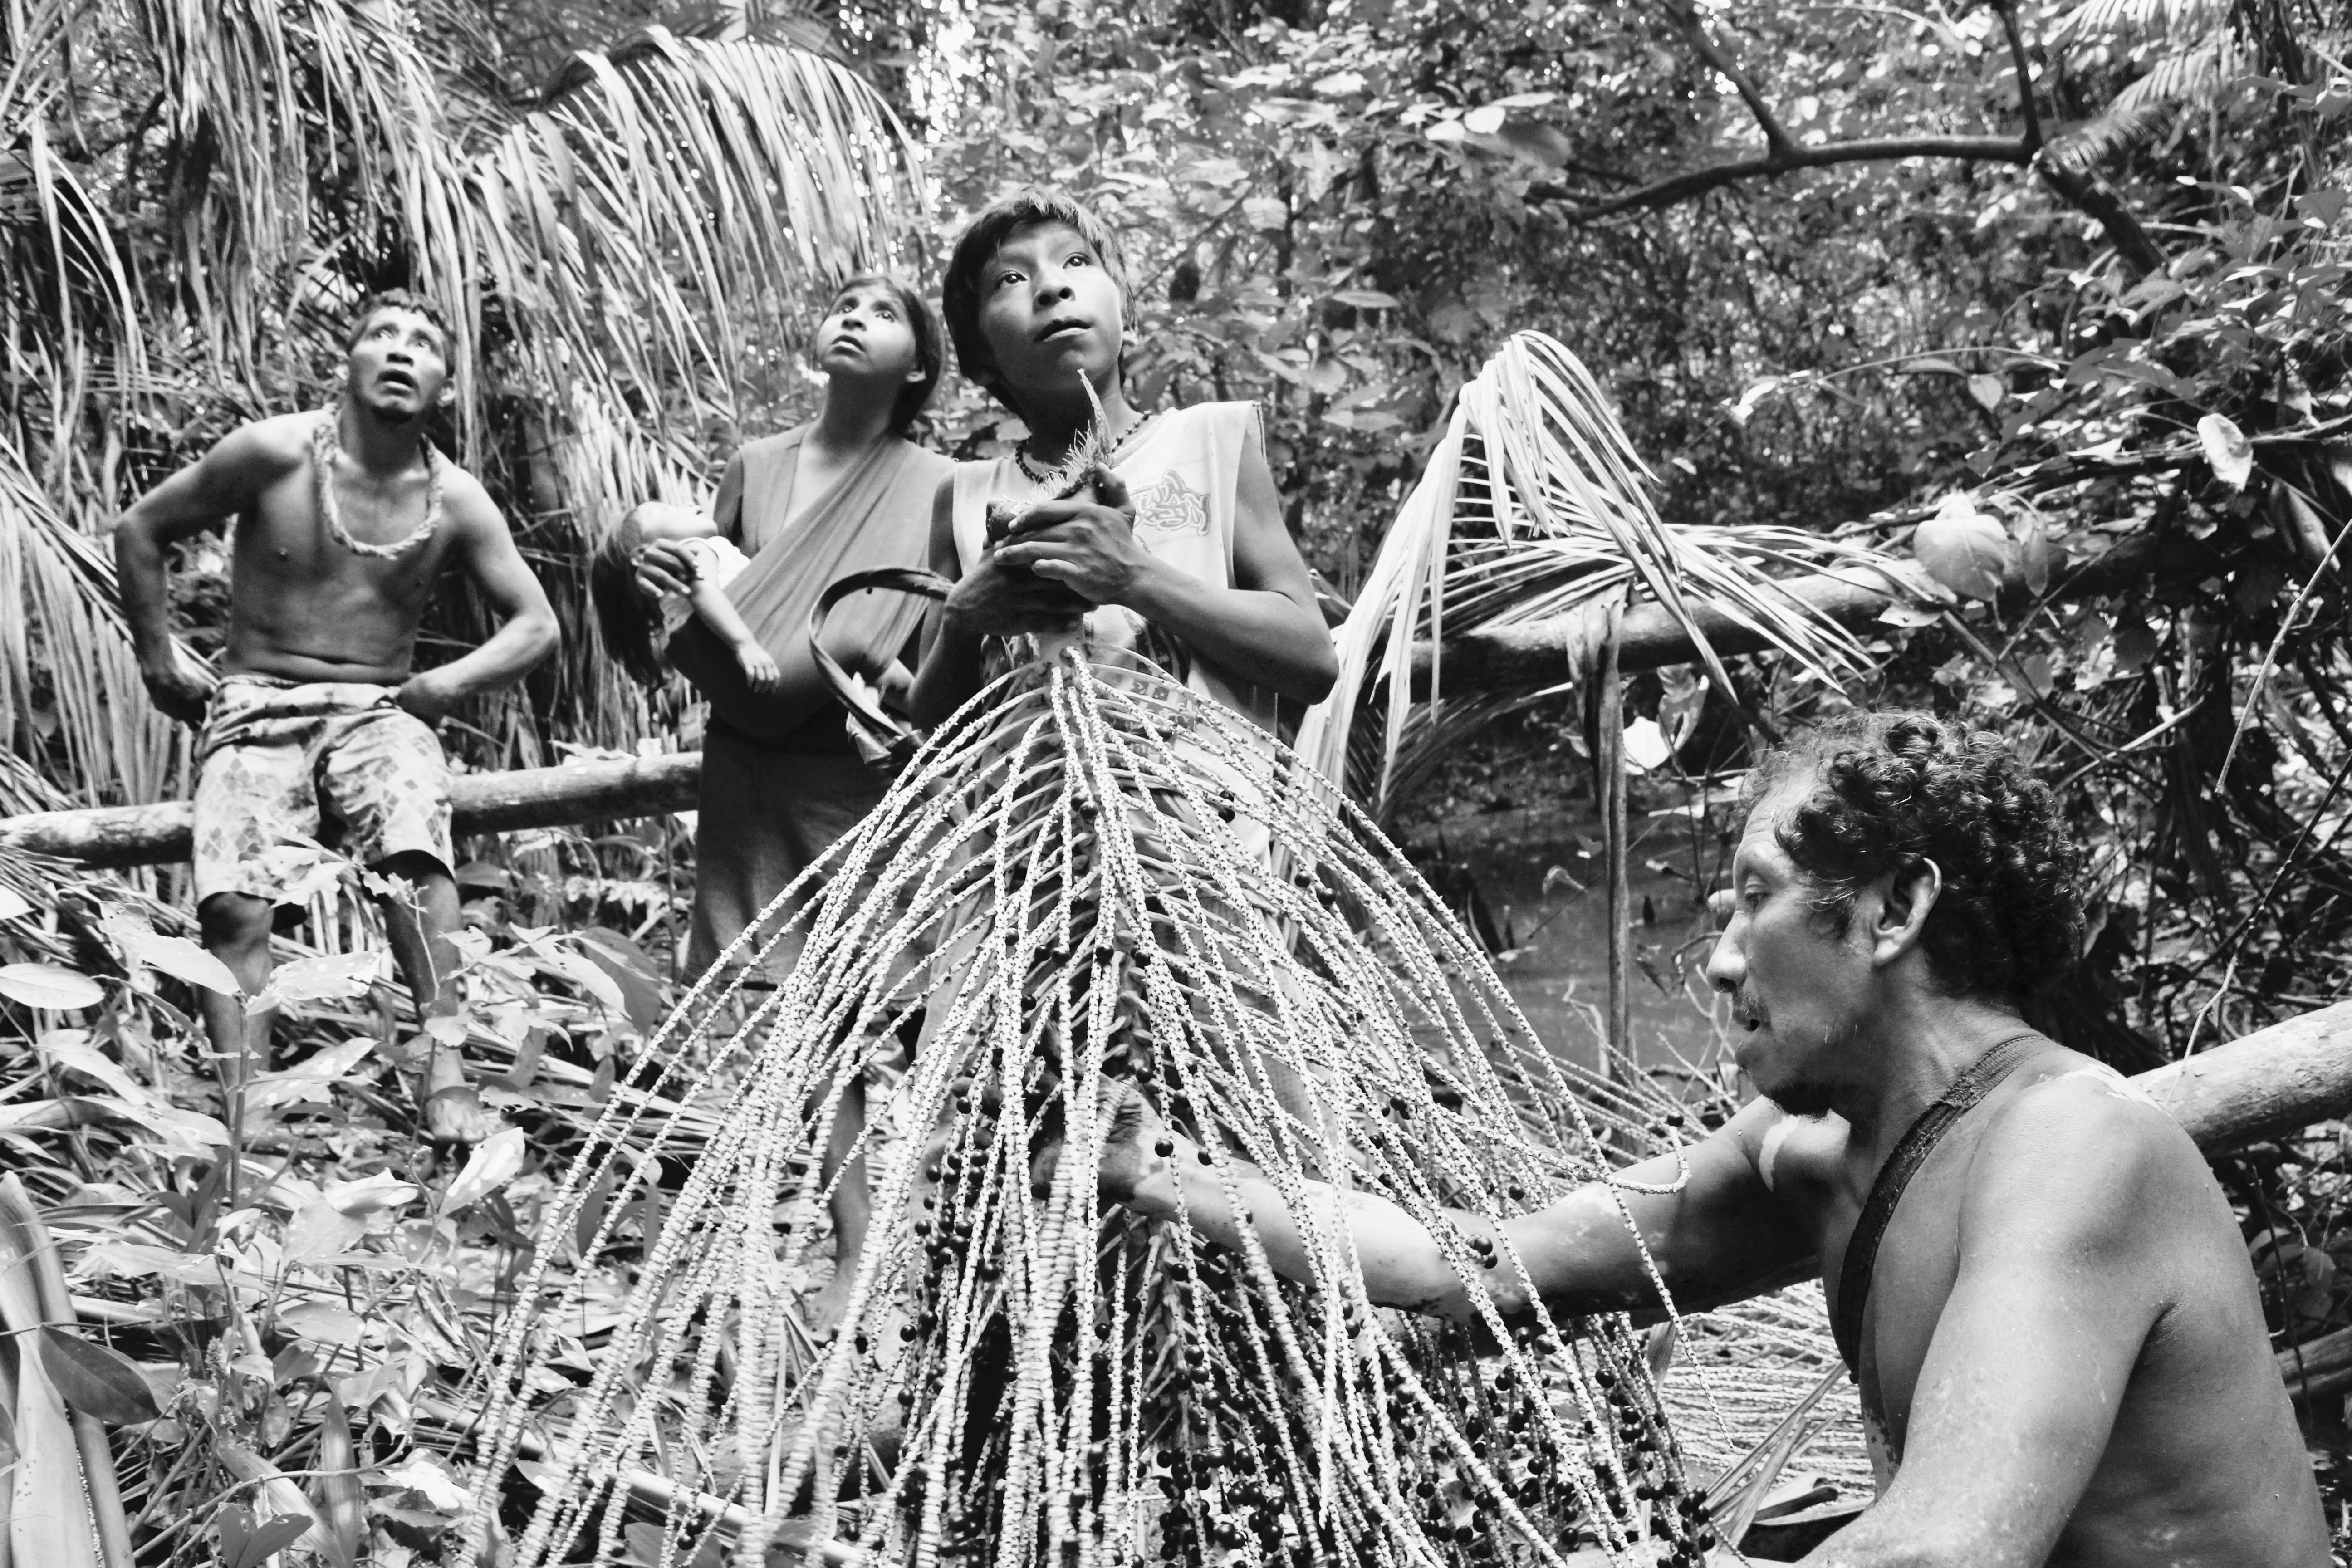
\includegraphics[width=\textwidth]{./imgs/IMG_2922}
\caption{(da esquerda para a direita) Jakara'yra, Makarikarỹa, Takwaripijua e Kamajrua
(agachado) colhendo juçaras na época das chuvas (aldeia Tiracambu, 2013).}
\end{figure}

\section{Palmeiras selvagens}

Dentre as etnografias que abordam a organização espacial de povos
amazônicos que encontram na caça uma atividade central, sejam
horticultores ou não (ver, por exemplo, o balanço de Rival, 1999), uma
das alegorias mais comuns é a do território como um espaço marcado por
histórias de caçadas e guerras, uniões matrimoniais e cisões entre
afins, nas que os saberes produzidos nas interações com a floresta
seriam, todo o tempo, colocados à prova e reinventados. São muitos os
exemplos: a paisagem supostamente caótica das florestas do Capauari, tão
familiares aos Ashuar, um ``território varado por mil acontecimentos''
que fornecem à paisagem aparentemente anônima sua devida substância
histórica (Descola, 2006, p. 153--154); os muitos topônimos existentes no
léxico Parakanã para situá"-los em suas trilhas, e pelos quais se
localizavam durante seus períodos de \emph{trekking} (Fausto, 2001, p.
105); o interesse dos Huaorani em sempre seguir adiante, por seus
caminhos, acompanhando o florescimento dos vegetais e o movimento dos
animais (Rival, 2002, p. 68); o ``seminomadismo'' Sirionó que, através
dos \emph{Ñenda}, os caminhos de caça, descobrem a cada caminhada uma
nova floresta, que lhes fornecerá as aldeias"-acampamentos em que vivem
(Holmberg, 1969, p. 105); a cultura material ``descartável'' dos nômades
Yuquí, donde os poucos objetos fabricados (cordas e cestos) são feitos e
refeitos de acordo com a necessidade, subprodutos exclusivos de sua bem
sucedida relação com a floresta (Stearman, 2001, p. 41); as complexas
descrições sobre o território realizadas pelos Akuriyó, levando"-se em
conta, fundamentalmente, a vegetação e a fauna, que coincidem com as
descrições presentes ``nas melhores enciclopédias de fauna e flora'' já
produzidas sobre o norte amazônico (Jara, 1996, p. 96). Enfim, em
variados contextos etnográficos sul"-americanos, entre povos para os
quais a caça desempenha um papel fundamental, que enfatiza um permanente
estar em movimento na floresta, a produção de múltiplos significados
sobre o território é condição primordial à existência da vida. São
espaços ``culturalizados'', nos termos de Ingold, cujas relações são,
antes, entre pessoas encarnadas em formas orgânicas, frágeis e não
permanentes (Ingold, 2000, p. 53), e nestes espaços a história está
escrita.

No capítulo que segue, apresento as formas pelas quais os Guajá concebem
e arranjam aquele que é seu lugar de vida: a floresta (\emph{ka'a}).
Para tanto, discuto a ideia de \emph{harakwaha}, termo que abrange tanto
o domínio territorial quanto as relações envolvidas no território. Ao
final do capítulo, apresento um pequeno esboço sobre a cosmografia
Guajá.

Como apresentei no capítulo anterior, os Guajá não têm uma economia
hortícola. Milho e mandioca foram introduzidos após o contato com o
Estado Brasileiro, e nenhum dos subprodutos de uma ``agricultura
tradicional'' indígena --- como fumo, beiju e bebidas fermentadas ---, tal
como encontramos em outros povos amazônicos (e os horticultores Tupi, em
particular), poderá ser encontrado entre os Guajá. Os espaços de vida
que constituem o território Guajá não contemplam a consagrada
espacialidade Tupi (e amazônica, de uma forma geral), que opõe a roça e
a mata como espaços"-eventos complementares em um ciclo sazonal. Como na
maioria dos grupos Tupi"-Guarani, o eixo céu"-Terra é um dos aspectos
fundamentais para entendermos a forma com que os Guajá se movimentam no
espaço --- embora haja exceções, como é o caso Waiãpi (Gallois, 1988).
\emph{Iwa}, \emph{haripa} e \emph{ka'a} --- ``céu'', ``aldeia'' e ``floresta'',
respectivamente --- são talvez os principais centros em torno dos quais a
vida gravita, formando pares particulares como ``céu"-Terra'';
``Terra"-mata''; ``mata"-céu'', que veremos daqui em diante. Céu e mata são
domínios pelos quais os Guajá guardam grandes interesses. Em boa parte
das conversas figuram como tema central, e eu não saberia afirmar sobre
qual as pessoas mais elaboram. A floresta, \emph{ka'a}, é o local em que
sempre viveram, \emph{habitat} de tudo o que conhecem: animais, mel,
remédios; apesar de todo o perigo que ela oferece, é o local que durante
sua história recente lhes forneceu a segurança e a distância necessária
dos \emph{kamara} e \emph{karai} --- os ``outros indígenas'' e os
``não"-indígenas'', respectivamente. Se não vivem mais baseados em
acampamentos, dormindo em tapiris como antes, não dispensam a vida na
floresta, local \emph{haxỹ} --- ``fresco'', e \emph{parahỹ} --- ``bonito''/
``bom''/ ``perfeito'', diferente da aldeia, que dizem ser \emph{haku} ---
``quente'' e \emph{manahỹ} --- ``desagradável''/ ``imperfeito''. Principalmente
no verão, a aldeia do posto é utilizada como base para novas incursões
de caça, e a caça é um dos principais assuntos tratados no dia a dia da
aldeia: munição, locais de caça, rastros de animais, etc., são os temas
que mais interessam. Os fatos da vida quase sempre são fatos da caça.

O \emph{haripa} (``minha casa'' ou ``minha aldeia''), nos dias atuais,
difere do que era antes do contato. Enquanto no passado os grupos
locais, formados por uma ou algumas famílias, viviam em aldeias
provisórias ou semipermanentes, refeitas devido aos deslocamentos
constantes dos grupos nos dias atuais, o que vemos são conglomerados de
antigos grupos locais que depois de amontoados se transfiguraram no
formato ``aldeia permanente'', devido tanto à proximidade com o posto da
Funai (que dispõe de bens e serviços) quanto ao maior conforto oferecido
por esta conformação espacial, sobretudo na época das chuvas. Os
pequenos acampamentos, próximos a áreas com grande oferta de caça e
frutos, deram lugar a grandes clareiras, com dezenas de casas onde vivem
até 180 pessoas (como no caso da aldeia \emph{Awá}), cada vez mais
distantes das áreas de caça. No entanto, por não se interessarem em
manter uma vida de cultivo nas roças, precisam voltar diariamente ao
mesmo interior da floresta onde outrora viviam. Andam para cada vez mais
longe, para onde a caça se foi, e precisam retornar à aldeia do posto,
tudo isso em uma única jornada. As aldeias, tal como hoje estão
organizadas, são espaços por um lado monótonos, dizem os Guajá, mas
dotados de vantagens, como a aludida proximidade com o mundo dos
\emph{karai}, e de uma estrutura fixa e funcional que os desobriga de
montar e desmontar seus acampamentos a cada poucos dias ou semanas. A
caça, por sua vez, devido ao desmatamento e à proximidade com os
brancos, está cada vez mais ``brava'' e por isso --- ao menos perto das
aldeias, locais de perturbação humana e barulhentos --- está mais difícil
caçar.

Como a grande maioria dos povos amazônicos, os Guajá não têm uma palavra
designativa para ``animal'', cada um é denominado por sua espécie, tipo,
tamanho ou outra característica. Na língua Guajá, no entanto,
encontramos um termo para ``caça'' ou ``presa'' que pode ser traduzido
também por ``bicho'': ``\emph{ma'amiara}'', ou simplesmente
``\emph{ma'a}'', seria essa palavra. A partir disso, fazem uma distinção
categórica entre ``caça brava'' (\emph{haitema'a}) e ``caça mansa''
(\emph{haite'yma'a}). Em linhas gerais, a caça brava é aquela acostumada
com o barulho dos tratores, motosserras, povoados, estrada de ferro e
presença dos humanos. A ``caça brava'' é mais atenta, desconfiada, enfim,
conhece os humanos e se torna mais difícil de caçar --- em oposição à
``caça mansa'', que são aquelas que vivem no interior da floresta, nas
áreas ainda preservadas. Nesses lugares, os animais estão menos
acostumados com a presença humana e vivem menos escondidos. Esses
``santuários'', verdadeiras ``reservas de comida'', são ocupados durante
todo o ano (com mais intensidade na época seca) e onde, como veremos
aqui, ainda se conseguem grandes quantidades de caça. As casas na
floresta, os acampamentos, são levantados nessas áreas, refúgio de
muitas espécies animais, longe das aldeias e dos postos indígenas. Lá a
caça fica perto das casas (acampamentos) além de existir em abundância.

\section{Seco e Molhado}\label{seco-e-molhado}

\subsection{\emph{Tamỹkoa} e a origem do verão}

\begin{quote}


\emph{\emph{Tamỹkoa} era um sujeito que morava na floresta e tinha os pelos
muito compridos. Seus cabelos (\emph{jakyra}) e barba (\emph{jamatara})
eram tão longos que se arrastavam por muitos quilômetros pelo chão. Os
pelos pubianos (\emph{hajmõ} \emph{kamỹtara}) eram tão compridos que
atravessavam a floresta inteira, bem como os cabelos das axilas
(\emph{jaura}), onde cada um seguia a direção de um braço, indo em
direções opostas até os recônditos daquele mundo. Até mesmo os pelos do
seu ânus (\emph{hajkarapyra}) era longuíssimos e sumiam pelos caminhos
da floresta. E os cabelos de \emph{Tamỹkoa} iam longe na floresta, cada
um em uma direção.}

\emph{Nessa época o herói cultural \emph{Maira}, o demiurgo que criou --- dentre
tantas coisas --- a própria humanidade, havia fugido junto com seu irmão
gêmeo \emph{Mukuxa'a} (o gambá), da aldeia das onças onde foram criados
como filhos e prisioneiros ao mesmo tempo. As onças haviam comido sua
mãe quando os gêmeos eram bebês e, quando cresceu, \emph{Maira}, após
descobrir a traição, conseguiu matar em vingança algumas onças, e fugir
com seu irmão, \emph{Mukuxa'a}, à procura de seu pai \emph{Mairua}
(\emph{Mai} ``\emph{Maira}'' + \emph{r"-ua} ``pai de''; literalmente o
``pai de \emph{Maira}''). Após um tempo de procura, \emph{Maira} e
\emph{Mukuxa'a} encontraram o pai vivendo na floresta. O encontro, no
entanto, foi mal sucedido, com Maira e \emph{Mukuxa'a} transformando o
arco do pai em cobra, e os quatis que \emph{Mairua} havia caçado foram
transformados em pedra\footnote{Voltarei à saga de \emph{Maira} no
  próximo capítulo.}. O pai de \emph{Maira} ficou muito bravo com seus
filhos e decidiu abandoná"-los, ou sair para caçar sozinho.}

\emph{Nessa época, \emph{Tamỹkoa}, o sujeito de pelos compridos, vivia nesta
mesma floresta. Durante sua caminhada, \emph{Mairua}, o pai dos gêmeos,
o encontrou dormindo. Quando o avistou, pensou: ``Ah, \emph{Tamỹkoa}
está aqui, dormindo!''. O pai de \emph{Maira} conseguiu passar por ele
sem acordá"-lo, seguindo o seu caminho. Logo atrás de \emph{Mairua}
vinham seus filhos, \emph{Maira} e gambá, que encontraram o rastro de
pelos de \emph{Tamỹkoa}. \emph{Maira} comentou com \emph{Mukuxa'a}, em
um falar sussurrado para não acordar \emph{Tamỹkoa}: ``Meu irmão,
\emph{Tamỹkoa} está dormindo para lá. Vamos pôr fogo em seus pelos
compridos, o fogo vai alcançá"-lo!''. E \emph{Maira} e seu irmão mucura
puseram fogo nos pelos de \emph{Tamỹkoa}. \emph{Mairua} a essa hora
estava bem à frente no caminho, e não imaginava que seus gêmeos iriam
segui"-lo, e muito menos atear fogo em \emph{Tamỹkoa}.}

\emph{O corpo de \emph{Tamỹkoa} se encontrava longe, muito longe deles, mas
seus pelos e cabelos eram tão compridos que os gêmeos perversos podiam
lhe tocar fogo à uma grande distância, a muito tempo de caminhada. O
fogo se espalhou pelos pelos de \emph{Tamỹkoa} e percorreu a floresta
inteira, passando o incêndio de um pelo ao outro. Tudo se queimou, como
um interminável caminho de fogo que secou o mundo todo. O incêndio
também secou os rios menores e os igarapés.}

\emph{\emph{Tamỹkoa} acordou sentindo um calor e, com a proximidade do fogo,
fugiu em desespero procurando algum curso d'água onde apagar o incêndio
de seus cabelos, mas estava tudo seco pois o fogo havia secado tudo.
Todos os seus pelos foram se queimando: o cabelo, os pelos das axilas,
pelos pubianos, do ânus, além da longa barba. Tudo foi queimado, e não
havia água para ele aliviar o incêndio. O incêndio secou a floresta.}

\emph{Enquanto \emph{Tamỹkoa} queimava, Maira e seu irmão, gambá, riam sem
parar. Depois de tanto procurar, e quase morrendo, \emph{Tamỹkoa}
conseguiu encontrar um rio, para onde se jogou, e vive dentro d'água até
hoje; nunca mais voltou à floresta com medo de morrer queimado.
\emph{Tamỹkoa} parece gente, como os \emph{awa}, mas vive com sua gente
embaixo d'água. Dizem que na época seca, quando os rios secam,
\emph{Tamỹkoa} pode ser visto pois gosta de tomar um pouco de sol, mas
sempre retorna às águas. Devido a esse grande incêndio que varou o
mundo, provocado por \emph{Maira} e seu irmão \emph{Mukuxa'á} (e a
contragosto de seu pai, \emph{Mairua}), até hoje, durante boa parte do
ano esses pequenos cursos de rios e igarapés ficam secos. (Narrado por
Hajkaramyykỹ).}
\end{quote}

\begin{center}
***
\end{center}

A estação chuvosa se inicia no final de dezembro, com intensificação do
volume das águas em janeiro, chegando ao máximo da cheia nos meses de
abril e maio, enquanto a seca, que se inicia em junho, tem seu auge no
mês de outubro. O calendário é bem dividido em duas estações, em que os
meses de dezembro/janeiro a junho são ``inverno'', e julho a dezembro,
``verão''\footnote{Para detalhes sobre o índice pluviométrico, dentre
  outros índices para as estações, ver Balée (1994, p. 9--10).}. ``Sol''
e ``chuva'', é assim que os Guajá se referem às duas estações do ano: o
inverno é chamado \emph{amỹna ky mehẽ}, literalmente: ``quando a chuva
vai'', e o verão é \emph{kwarahy mehẽ}: ``quando tem sol''. E as pessoas
guardam sentimentos e percepções bem diferentes sobre cada uma delas.

Em uma tarde de março, no inverno de 2008, a chuva invadia a casa de
Wiraho. As folhas de babaçu, colocadas um ano antes e substituídas
apenas em alguns pontos, não eram suficientes para aplacar a força da
água. Embora o telhado conseguisse abrandar o vigor da chuva, tivemos
que recombinar nossas redes para que as goteiras da casa não tirassem
nosso conforto. Trovejava bastante. ``São os \emph{tapỹna}!'', me disse o
jovem Juwi'i. ``Estão com muita raiva (\emph{imahy}, ele está com
raiva), eles sempre estão \emph{brabos}'', disse"-me o velho Pirama'ã,
antes de começar a entoar a canção de um \emph{karawara} chamado
\emph{Takwari} \emph{pini'ĩ} --- uma ``gente taquarinha'' que vive no céu,
cuja canção atemoriza os \emph{tapỹna}. Por isso, sempre que os
\emph{tapỹna} estão nervosos e na Terra se ouve o barulho de seus gritos
--- os trovões \emph{tapỹna} --- deve"-se cantar: \emph{takwaaariiii}
\emph{pinĩĩĩĩ}, \emph{takwaaariiii} \emph{pinĩĩĩĩ}, até que os trovões
se acalmem. Se para de trovejar é sinal de que os \emph{tapỹna} ouviram
os humanos e se acalmaram. No moquém (\emph{pakapa'ã}) havia um pequeno
pedaço de cotia (\emph{akwixia}) que alguém caçara no dia anterior,
porém todos sentíamos alguma fome. Em meio a essa situação, com as redes
úmidas e os animaizinhos de criação encolhidos pelo frio de inverno, eu
conversava com Wiraho e Piraima'ã que me diziam que, com exceção do
aumento de gordura (\emph{ikira}) de muitos animais durante a época da
chuva (o que é ótimo), preferem o verão (\emph{kwarahya}), quando não
sentem frio, podem andar livremente e dormem na mata.

Por ser no período chuvoso que grande parte das plantas frutifica,
\emph{a'e} \emph{ja'akera} --- ``tem fruta!'', é esta também a época de
engorda dos animais \emph{ikira ra'o} --- ``muito gordos''. De acordo com
Cormier, enquanto 95\% dos frutos aparecem na estação chuvosa, esse
número cai para 43,9\% durante a estação seca (Cormier, 2003, p. 47).
Nesta época, após abater uma presa, as pessoas realizam pequenas
incisões no animal (principalmente aqueles que só engordam no inverno,
como macacos e quatis) com o auxílio de galhos de árvore ou mesmo facas,
curiosos para verificarem o quanto de gordura escapará por esses
orifícios. Quanto mais gordura conseguem encontrar nestas pequenas
amostras, maior será o prazer que terão à mesa. Capelães, diversos
macacos, queixadas, caititus, antas, cotias, quatis, pacas, além das
diversas aves (algumas espécies de inhambus e jacus, além de
mutuns"-cavalo e jacamins) estão repletos de gordura devido aos frutos da
estação --- \emph{amỹ kiraha} ``gordura da chuva'' --- disseram"-me certa vez,
quase como inferindo que a gordura é uma consequência natural das
chuvas. O inverno, por isso, é o tempo da gordura, de uma maneira geral
\emph{ma'a ikira} ``a caça está gorda'' e, antes de tudo e de maneira
específica, o tempo do ``capelão gordo'', da gordura do capelão
(\emph{wari kaera}) que --- de uma apetitosa cor amarelo ouro --- se
esparrama do animal ventre afora, após os furinhos que fazem ainda nos
locais de caça.

Mas não é só da gordura do capelão que vivem as pessoas durante o
inverno. Abate"-se uma grande quantidade de outros animais, como cotias e
pacas, alimentos quase que cotidianos e encontrados em abundância na
região dos rios Caru e Pindaré. Durante minhas estadas em campo, a
quantidade de cotias e/ou pacas consumidas era similar ou mesmo superior
à de capelães, sem paralelo com nenhum outro animal (me refiro aos
indivíduos da espécie que são caçados, e não à quantidade de carne
total). Como exemplo, em um acampamento de quatro noites realizado no
final da estação das chuvas com pessoas da aldeia juriti, foram abatidos
10 capelães e 12 pacas (além de outros animais). Em muitas épocas --- de
seca ou de chuva --- pacas e cotias garantiam a segurança alimentar, mais
do que os próprios capelães.

No inverno, a gordura é tanta que, ao limparmos animais de médio e
grande porte (fosse uma paca ou um caititu), ela saía em grandes blocos,
junto com as próprias vísceras. Ao apresentar a estação chuvosa nas
matas do Capauari, Descola observa que essa é a `` `época da gordura do
macaco"-barrigudo', em referência à bela camada de banha que o animal
passa a acumular no torso'':

\begin{quote}
\emph{Aqui, como em boa parte do mundo ameríndio tradicional, a gordura é
escassa devido à falta de animais domésticos, e se torna muito cobiçada
por serem poucas as oportunidades de comê"-las. Este gosto pela gordura
vai além das meras exigências do metabolismo, e traduz o valor que essas
sociedades atribuem à corpulência e às carnes rechonchudas como sinais
de saúde e beleza (Descola 2006, p.170---171).}
\end{quote}

É pela fartura, e não pelo conforto, que a estação das chuvas é
apreciada. O ``verão'' é uma época melhor para se mover na mata, porém a
caça é magra. Além do capelão gordo, a maioria dos frutos
(\emph{ja'akera}) aparece na época das chuvas: bacaba, cupuaçu e pequi
marcam a estação.

Nos dias de hoje, quando não estão aplicados nas atividades de roça e
pomares coordenadas pela equipe da Funai, seu inverno é passado entre a
aldeia e a mata. Antes do contato, essa era a época em que cada grupo
local se isolava, viviam em separado até o fim das chuvas. Se os Guajá
se organizavam em grupelhos --- compostos por algumas famílias aparentadas
--- dispersos sobre um grande território, era na época da chuva que tais
grupos se encontravam ainda mais reduzidos demograficamente, compostos
muitas vezes por apenas uma família nuclear. O sucesso das sucessivas
mudanças de aldeia era proporcionado pela pequena escala populacional
envolvida nos deslocamentos. Quanto menores as aldeias, menores eram os
impactos no novo sítio. Os lugares para as novas aldeias de inverno
também deveriam ser bem escolhidos, pois, como me disseram, quando
viviam na floresta, muitos Guajá morreram esmagados por troncos que caem
das árvores, derrubados pelos ventos e pelas chuvas. Durante o inverno,
muitas rotas (\emph{-pea} --- ``caminho'') são intransitáveis, devido ao
alagamento de brejos e rios para pessoas que só se locomovem por
trilhas, pois até o contato não conheciam canoas\footnote{Desde o
  contato com a Funai uma geração mais jovem, que cresceu perto dos
  postos (e hoje está na faixa dos vinte cinco anos), já possui certa
  familiaridade com canoas e muitos sabem nadar, diferente dos que estão
  acima dos trinta anos.}, o que representa uma significativa limitação
às atividades sobre o território. A formação de diversos igapós,
resultantes dos alagamentos, em vez de propiciar uma vantagem
estratégica para caçar --- uma vez que limitaria a área vital de todos os
animais, tal como ocorre entre povos canoeiros (ver o caso Pirahã,
Gonçalves, 2001, p. 83--122) --- representa o fim de suas trilhas, que
durante a estação molhada são completamente inutilizadas. São esses
pequenos desconfortos, inerentes ao cotidiano do inverno, que fazem
desta uma estação pouco apreciada pelos Guajá.

Os Guajá não reclamam de uma penúria proteica durante as chuvas, como
ocorre entre os Pirahã (Gonçalves, 2001, p.123--133), tampouco dizem
explicitamente que é uma época desconfortável, ainda que a chuva assim a
torne, pelo menos para mim --- é desconfortável, úmida e bolorenta. Como a
``floresta está molhada'' (\emph{ta'amuhũ ka'a}), as muitas ladeiras
(\emph{wytyra}) que formam o território ficam escorregadias e os
igarapés transbordam, dificultando a travessia. Espinhos, cipós
espinhosos e úmidos, cortes que não cicatrizam e muita lama. Os caminhos
que conhecemos no verão desaparecem e cedem lugar a lagos, lagoas e
brejos. Apesar de tudo isso, os animais parecem não se importar. 
Com exceção do caprichoso capelão, que detesta se molhar e se
esconde nas folhas até o temporal dar uma trégua, os porcos, caititus,
antas e toda a macacada continuam a circular, agora molhados,
permanecendo na mata. Como as bacias do Gurupi e Pindaré são
entrecortadas por diversas serras (Serra do Tiracambu, Serra da Desordem
e suas tributárias), os Guajá viviam quase que o ano inteiro nessa
extensa área de terra firme, fosse na estação chuvosa ou no verão, e como não necessitavam de roças para
viver, as \emph{wytyra} (``montanhas''), regiões íngremes e muito
preservadas em fauna e flora, lhes ofereciam tudo de que precisavam.

Ainda hoje fazem acampamento na estação chuvosa. \emph{Ka'a ta'amuhũ},
``a mata molhada'', apresenta mais dificuldades, seja para montar um
acampamento ou caminhar. Na caminhada, que pode durar até três dias,
entre a aldeia e o acampamento --- a ``casa na floresta'' (\emph{ka'a
ripa}) ---, é necessário parar diversas vezes durante o percurso e esperar
a chuva estiar. Os abrigos são feixes de folhas de palmeira (açaí, por
exemplo) amarrados em troncos de árvores em forma de pequenos avancês,
muito provisórios, mas capazes de proteger perfeitamente seu ocupante
das gotas grossas que são acumuladas nas árvores. Nas caminhadas, passam
de um morro a outro apenas margeando seus contrafortes e voltam a subir
uma nova colina. Algumas passagens são praticamente verticais, como
escadas, subidas íngremes formadas pelas raízes das árvores. Caminham no
mato assobiando de tempos em tempos a fim de atrair emplumados, como
azulonas, inhambus e jacupembas. Tais animais, dizem os Guajá, cantam
pouco na época do inverno, e os homens os imitam para ouvir suas
repostas e, eventualmente, caçá"-los enquanto se deslocam.

Os dias nos acampamentos de inverno são pacatos. Enquanto os homens saem
para caçar, as mulheres permanecem com seus filhos, mantendo o fogo
aceso e o estoque de lenha seco e abastecido para aquecer os corpos
durante as noites frias. No verão, por ser mais fácil andar na floresta,
as mulheres (sobretudo as de casais jovens e apaixonados) costumam sair
do acampamento e se juntar aos companheiros em caçadas. Podemos, no
entanto, afirmar que existe uma espécie de divisão das tarefas nas casas
da floresta: os homens vão caçar, e as mulheres cuidam da comida e da
manutenção do acampamento. Não quero, contudo, advogar por uma projeção
automática entre esferas doméstica e selvagem em que homens e mulheres
dividiriam de maneira complementar suas funções (Strathern 1980). Mais à
frente veremos como a participação das mulheres na caça embaralha
qualquer tentativa simplista de correlacionar campos aparentemente
opostos, como \emph{aldeia e floresta}, \emph{natureza e cultura}, no
universo Guajá.

Nas casas na floresta come"-se bastante durante o dia. Uma parte grande
do que é caçado, porém, é separada para ser levada à aldeia. Os
acampamentos servem para isso também, formação de um estoque de comida
que posteriormente será repartida a um coletivo mais amplo, na aldeia.
Os Guajá permanecem durante semanas na floresta, acumulando grande
quantidade de carne moqueada. Nas chuvas, o cheiro de gordura defumada,
terra e folhas molhadas é o que sobressai nos acampamentos --- junto com
as risadas das crianças, que não param de mastigar. Permanecer na
floresta durante as chuvas é observar uma paisagem úmida e esfumaçada,
proveniente da evaporação da umidade no solo, troncos e árvores. Os
acampamentos de inverno ficam próximos dos acessos a igarapés, porém
normalmente instalados no topo de um morro, no conforto das ``terras
altas'' (\emph{wytyra}), mais seguras, drenadas e limpas, como sempre
preferiram. Mulheres e crianças quando vão tomar banho abastecem o
acampamento com água para cozinhar, lavar a louça ou dar banho em bebês
--- hoje em dia trazem tudo em garrafas pet. É diferente do verão, quando
acampam às margens dos igarapés (\emph{ipio}), com as pessoas indo e
vindo da fonte d'água. Já no inverno, todas as áreas no entorno dessas
fontes estão alagadas.

Mesmo com o sol a pino, por volta das 10 da manhã, as gotas continuam a
cair pelas folhas e cipós das árvores encharcadas. O sol brilha sobre as
árvores, mas o chão, assim como as casas do acampamento, permanece
encharcado. Todo o chão da floresta, as folhas e os troncos úmidos se
agitam emitindo uma fumaça, algo neblina, algo vapor. Mesmo com o sol a
pino no meio da manhã e a atmosfera quente acima das árvores, dentro da
floresta as gotas continuam a escorrer pelas folhas e cipós das árvores
ensopadas, tal como pontos luminosos, a nos lembrar que, mesmo em dias
ensolarados, para a floresta ainda é tempo de chuva. O inverno é assim,
um som interminável de gotas a cair sobre a mata. Após os dias vividos
na mata embaixo de chuva, protegidos pelas grossas palhas dos tapiris
com as roupas e redes úmidas, sentindo o frio e desconforto (mas comendo
bastante gordura), as centelhas de sol permanecem entre as árvores, cada
vez mais secas. O tempo começa a se abrir e esquentar. O inverno está
chegando ao fim.

A grande dispersão do inverno contrastava com a concentração do verão.
Um tempo ``seco'' --- \emph{ikỹ}, em que ``a floresta vai secar''--- \emph{ikỹ
ta ka'a}; quando os rios estão secos, \emph{tapa y'a} --- ``a água seca''.
Originalmente, era uma época em que diferentes grupos locais, ligados
por laços de parentesco, corresidiam em aldeias um pouco maiores que as
de inverno, quando caçavam (\emph{wata}), cantavam (\emph{jã}) e viviam
juntos (\emph{ikwẽ e pyry}, ``permanecer junto''). As aldeias de verão
funcionavam como grandes aldeias bases, constituídas quase que
totalmente por tapiris (\emph{tapãj}) em número proporcional às famílias
e um ou dois moquéns, onde a comida era preparada. A partir dessas
aldeias de verão --- que podiam ser constituídas, por exemplo, por um
grupo de germanos e sua prole --- todo o território era explorado, o que
dava origem a outros pequenos e (ainda mais) provisórios acampamentos,
formados por grupos ainda menores, a partir de uma só família ou mesmo
um jovem casal\footnote{Como veremos no próximo capítulo, embora boa
  parte dos casamentos seja intergeracional, é possível encontrarem"-se
  casais compostos por jovens de idades próximas.}. Tributários desta
aldeia maior, os microacampamentos de verão se localizavam a até alguns
quilômetros de distância da aldeia acampamento base e se justificavam
quando as pessoas seguiam por dias a fio o rastro de uma vara de
queixadas ou iam explorar uma região rica em macacos ou bacabas, dentre
outros motivos.

Nos dias atuais, durante o verão montam acampamentos na floresta onde
podem permanecer por várias semanas (ou até meses) --- algo que fazem com
menos frequência a cada ano\footnote{Pude encontrar nos relatórios das
  frentes de atração menções aos primeiros anos de contato, quando os
  grupos recém"-contatados passavam períodos de até seis meses em
  acampamentos na floresta e retornavam esporadicamente ao posto. Hoje,
  tais períodos não passam de algumas semanas, e durante meu tempo de
  trabalho de campo nenhuma família passou mais do que um mês em uma
  dessas aldeias de verão.}. Do ponto de vista econômico"-alimentar,
estas seriam as principais diferenças entre as duas estações. No verão,
menos gordura, mais caminhadas e vida concentrada na mata, enquanto que
os meses de inverno são passados entre os acampamentos, a aldeia do
posto indígena, e a mata, com muitas trilhas inutilizadas devido à cheia
de rios (\emph{y'ruhua}), brejos (\emph{ta'amuhũ pãj} ``está tudo
alagado'') e igarapés (\emph{ipio}), além do aparecimento de inúmeros
igapós.

Para além da economia e ecologia, os Guajá defendem que as mudanças
estacionais são de ordem cosmológica, uma variação sazonal na composição
do universo, proporcionada em parte por arranjos de alguns de seus
habitantes celestes. A chuva é controlada no céu (\emph{iwa}); este é um
local que possui um grande ``reservatório'' de água quente, que compõe o
primeiro patamar celeste. O reservatório estaria repleto durante certa
época, e sua água transbordaria para a Terra (\emph{wya}) em forma de
chuva, originando"-se daí o inverno (\emph{amỹna}, ``chuva''). Não poderia
afirmar com exatidão que tipo de controle é exercido sobre essas águas
celestes (nem mesmo sei se seu fluxo para a Terra é totalmente
controlado); de toda forma, recebi algumas explicações sobre o fenômeno.
Em uma delas, quem controla as águas caídas deste reservatório celeste é
\emph{Maira} --- o demiurgo criador da humanidade (\emph{awa}) e de boa
parte das coisas que estão no mundo. Ele teria acesso a uma espécie de
``torneira'' --- assim disseram para que eu entendesse\footnote{Durante o
  tempo que passei entre os Guajá para me explicarem os fatos de ``seu mundo'', as pessoas gentilmente utilizavam imagens do ``meu mundo'' (como
  {torneiras}, {espelhos} e {motores}) para que eu entendesse as
  explicações. Boa parte da tese que originou este livro está baseada em
  explicações que me foram fornecidas nestas formas transnominadas, que
  em alguns momentos, como agora, eu não poderei deixar de transcrever
  fielmente.} --- que controlaria conforme o primeiro patamar celeste
estivesse repleto de água. Outra explicação me foi dada nos meses finais
de campo, quando me disseram que o controle das chuvas era feito pelos
\emph{karawara}, a principal categoria de seres celestes que povoam o
\emph{iwa}. Os \emph{karawara}, por serem também caçadores de animais da
Terra (\emph{wya}) e que os levavam para serem consumidos no céu
(\emph{iwa}), controlariam a quantidade de chuva durante o inverno, de
acordo com suas sucessivas vindas à Terra para caçar, extrair mel,
buscar água fresca (já que a água celeste é imprópria para o consumo,
como veremos), dentre outras atividades terrenas. Os Guajá explicam que
a chuva cessa quando os \emph{karawara} ``desligam a torneira'' e descem
para caçar; e assim que voltam para o céu fazem a água cair novamente.

A situação cósmica se modifica durante o \emph{kwarahya} (verão), quando
o céu pode ser visitado pelos humanos. Durante o \emph{kwarahya, Maira}
se ausenta dos patamares celestes mais próximos e se dirige a uma região
situada a leste no céu, quando vai passar uma temporada na aldeia dos
parentes de sua esposa --- seus cunhados e sogros (\emph{harapihianã}) --- e
retorna apenas no inverno. É no \emph{kwarahya} que o fluxo de água
celeste, \emph{amỹna}, que cai na Terra durante o inverno, é
interrompido, permitindo que os humanos possam ir ao céu cantar com os
\emph{karawara}, e que essa gente celeste possa vir à Terra cantar com
os humanos. Se não existisse o tempo da estiagem, não existiria o
trânsito de humanos para o céu, através da \emph{takaja} (o abrigo
ritual). A água celeste é destruidora por natureza, pois (1) deve ser
constantemente equilibrada, e as estações de chuva e seca são a
consequência natural deste equilíbrio, além de (2) ser, por si só,
perigosa pois, por ser ``vermelha'' (\emph{pinỹ}) e ``quente''
(\emph{haku}), é nociva aos humanos que se encontram na Terra. Durante
sua queda na forma de chuva, a água celeste passa por um processo de
esfriamento (\emph{haxỹ}) até chegar à Terra, tornando"-se benéfica ou,
ao menos, não"-nociva. A água que escorre do céu na estação chuvosa é
proveniente desta grande água celeste, \emph{iwa 'ya} (``água do céu'').

Diferentemente do que encontramos em outras paisagens Tupi"-Guarani, os
Guajá não fornecem qualquer narrativa sobre um ``dilúvio universal'' que
tenha dado origem ao mundo atual ou porvir (ver Clastres, 1978, p.
24--26; e Nimuendaju, 1987, p. 67--71). Como veremos mais adiante, outrora
os diversos patamares celestes, a Terra, e o mundo subterrâneo eram
muito próximos (algo semelhante à escatologia Araweté). O surgimento da
Terra (\emph{Wy}) se dá quando, num momento, ocorre a separação desses
patamares. Porém, não se descarta a ideia de que o controle da água
celeste exercido por \emph{Maira} (e/ou pelos \emph{karawara}) esteja
relacionado com o tema da ``água destruidora'', presente em outros povos
Tupi"-Guarani (ver Viveiros de Castro, 1986, p. 197--204).

\section{Na água}\label{na-uxe1gua}

Tal como os Parakanã e os Araweté --- como já dissemos --- os Guajá podem
ser considerados um povo de cabeceiras de rio, cujo deslocamento, no
verão ou no inverno, apesar de todo o alagamento da área, era realizado
sem o auxílio de qualquer embarcação. Vieram a conhecer canoa após o
contato, quando a Funai passou a comprá"-las e oferecê"-las às
comunidades. Ainda hoje, apesar de que as gerações mais jovens saibam
navegar, desconhecem qualquer técnica de fabricação de canoas. Homens
com mais de 40 anos não têm qualquer desenvoltura com o remo, e os que
sabem nadar com alguma segurança são mais jovens. Como também aponta
Fausto para o caso Parakanã, os rios dessa região ``não eram vias de
comunicação, mas antes obstáculos naturais que eles procuravam franquear
ali onde se estreitavam ou tornavam"-se mais rasos, em particular durante
a estiagem'' (Fausto, 2001, p. 106). Os Guajá, com exceção das crianças
em alguns horários do dia, não frequentam os rios e muito menos aprovam
a ideia de ser um local onde se possa ficar muito tempo tomando banho e
se divertindo, dentro ou fora d'água. O local onde se regozijam de
prazer e alegria e passam muitas horas do dia, simplesmente deitados ou
conversando, é a densa floresta; preferem o banho em cursos mais rasos,
opacos e desconfortáveis do que em partes mais caudalosas e cristalinas
--- e por isso achavam graça no meu aparvalhado prazer em dar mergulhos e
braçadas nas partes fundas do rio Caru, acompanhado das crianças.

Se tirarmos pelos muitos casos de afogamento seguidos de morte que já
ocorreram e por não se sentirem à vontade nessas águas, fica evidente
que os rios ('\emph{ya}, ``água'') não são locais de prazer para os Guajá.
E, ao contrário de outros povos, não precisam dos rios para nada, tendo
em vista que, até o contato, não navegavam; caçavam muito mais que
pescavam e não precisavam de suas águas nem para pubar uma carga de
mandioca. Um pequeníssimo igarapé, ou mesmo uma área alagada, era
suficiente para lhes fornecer água de uso e algum peixe.

A água que bebem na mata é retirada de cacimbas à beira desses pequenos
cursos d'água (hoje, a aldeia Juriti possui uma bomba d'água e outras
aldeias chegam a ter caixas d'água). Durante nossas caminhadas, passando
pelos igarapés, encontrávamos cacimbinhas antigas que, ao serem cavadas,
eram facilmente reativadas. No entanto, elas forneciam uma água um pouco
mais turva que a do rio. Ao serem indagados sobre o porquê de escolherem
beber (algumas vezes) a turva água da cacimba em vez (algumas vezes) da
água cristalina do rio, explicavam que a água do rio é aparentemente
limpa, porém repleta de dejetos de animais, além do fato de muitos
bichos morrerem no rio e poluírem suas águas, enquanto a água da cacimba
é bastante segura, já que não mantém contato com o rio. Certa vez, Anĩa,
a pequena filha de Hajmakoma'ã, ficou muito doente com um quadro viral:
febre, garganta inflamada e dor de cabeça, e foi tirada às pressas da
aldeia sob o risco de morrer. Hajmakoma'ã explicou"-me que ela estava
sempre tomando água diretamente do rio e que ``a água do rio faz mal''.

O rio como um obstáculo a ser transposto nunca cedeu lugar ao rio como
uma via de locomoção. Na aldeia Juriti, nos dias de hoje, algumas
pessoas se interessam em pilotar pequenos motores de popa (os populares
``rabetas'') nas imediações da área do posto a fim de acessar algumas
áreas de caça e pesca rio abaixo, mas não se aventuram a ir muito longe
devido à presença de não"-indígenas na região. Ao mesmo tempo, na aldeia
Tiracambu, os jovens, atraídos pelo povoado que se encontra bem próximo
à outra margem do rio, enfrentam a correnteza do médio Pindaré remando.
As canoas são de diversas procedências: voadeiras de metal compradas com
recursos do governo; canoas de madeira compradas de barqueiros da
região; e até pequenas canoas apreendidas em operações contra
madeireiros ilegais que sobram como espólio do posto indígena e são
utilizadas pelas comunidades. Mesmo que os jovens estejam aprendendo a
navegar, o que pode representar o início de uma mudança na relação dos
Guajá com os rios, em março de 2009, durante o inverno, em uma grande
cheia que ocorreu em boa parte do estado do Maranhão e Pará, Pinawãxa'a
morreu afogado ao cair de sua canoa quando coletava ingás para seu
sobrinho, nas imediações do posto. Com cerca de 40 anos de idade, ele
não sabia nadar e ao cair n'água com o rio cheio não conseguiu
sobreviver. Vale notar que os rios e igarapés da região não são largos
nem caudalosos em relação a outros rios da Amazônia. Se comparado com
rios médios da bacia do Amazonas ou Tocantins, o rio Caru, que margeia a
aldeia Juriti, não passaria de um pequeno curso d'água!

Tal como os topônimos que marcam os pontos da floresta, os rios podem ser nominados 
e '\emph{ya} (``água'') é a forma utilizada para se
referirem a eles. Algumas vezes, quando perguntava o nome de pequenos
igarapés que encontrávamos no curso de nossas caminhadas, diziam se
tratar de um igarapé chamado ``\emph{Jaku}'' (jacu), ``\emph{Jawara}''
(onça), ``\emph{Mitũ}'' (mutum), pois os Guajá nomeiam os rios e igarapés
a partir de circunstâncias ou de uma característica ali presente. Um
igarapé tributário do rio Pindaré é chamado \emph{Ajỹ} \emph{nima} (ser
de criação dos \emph{ajỹ}), pois é um local que os \emph{ajỹ}
frequentam. Ou o igarapé '\emph{Y itatuhuma'a}, ``rio cheio de pedras''.
Outro curso d'água é chamado \emph{Amiriy'a}; \emph{amiria} é um
peixinho, ``rio do \emph{amiria}''. Ou outro chamado
\emph{Wirapehepehena}, cuja tradução pode ser  ``Pau quebrado dentro'',
provavelmente por algum evento passado. Os igarapés menores, em geral,
são chamados \emph{ipio}, já um igarapé grande, como o igarapé do
Presídio, pode ser chamado '\emph{yruhua}, literalmente ``água/rio
grande''. Tais nomes de rio eram muito mais uma alusão a eventos que
ocorreram no local, determinados pelo substantivo nomeador ligado à
história do local (os vestígios de uma onça; a caçada a um mutum, etc.)
que consequentemente se desdobrava em um topônimo. Muitos, no entanto,
eram conhecidos por um ou outro grupo de pessoas que viveram uma
história no local, por isso geralmente os nomes de muitos igarapés não
seriam nomes próprios, diferentemente de como fazem os
não"-indígenas\footnote{Desta forma os igarapés ``Juriti'', ``Mão de Onça'',
  ``Turi'', ``Preto'', dentre tantos que compõem a bacia da Caru --- alguns
  dos quais constam como parte dos marcos naturais da terra indígena
  \emph{Awá} ---, não são reconhecidos pelos Guajá por esses nomes. E, por
  exemplo, um certo ``Igarapé da Onça'' conhecido pelos Guajá é o mesmo
  ``Mão de Onça'' conhecido pela Funai, o que causa certa confusão no
  diálogo das pessoas da aldeia com os funcionários do posto. Foi o caso
  de uma estrada ilegal, aberta recentemente, que corta o ``Igarapé da
      Onça'' dos Guajá e fica a uma distância de 6 km da aldeia, e não o
  ``Igarapé Mão de Onça'', cujo nome é dado pelos \emph{karai}, e se
  encontra muito mais afastado da aldeia.}. O rio Caru, o principal na
aldeia Juriti, é chamado simplesmente de '\emph{Ya} (água) --- ou
\emph{Karu 'Ya} ---, referindo"-se à denominação dada pelos \emph{karai}
(não"-indígenas). Mais do que por meio de nomes próprios, os Guajá
indicam as relações entre rios, igarapés e pequenos cursos d'água por
termos de cognação, que exprimem relações de parentesco reais. Portanto,
um igarapé pode ser \emph{imymyra} (``filho dela'') de um rio, e um
pequeno curso d'água pode ser o \emph{-nima} (``ser de criação'') do rio.
Estas eram as formas usuais e constantemente utilizadas que me contavam
para explicar de onde provinham determinadas lagoas (\emph{ta'amuhũ pãj}
``alagado'') e igarapés (\emph{ipio}), dentre outras dúvidas procedentes
quanto ao caminho dos rios.

Houve uma época em que, segundo eles, os rios e seus habitantes não
existiam. Os rios e igarapés foram abertos ``como se abrem estradas'' por
um jacaré (\emph{jakare}) comedor de humanos, grande e perigoso. Esse
jacaré, que era tão largo quanto uma estrada, derrubava árvores e por
onde passava abria o caminho pelo qual a água chegaria. Um homem me
disse que a técnica é parecida com a dos tratores que ``puxam'' uma
estrada, como as tantas que já encontraram ilegalmente abertas em seu
território. Foi este jacaré gigante que, após abrir os caminhos que
vieram a ser os cursos dos rios, inundou"-os com água e os formou,
finalmente. O jacaré tinha uma aparência humana, ``um jacaré sem rabo e
com a pele como a nossa, como a de um Guajá'', me contou um Wiraho certa
vez.

Quanto aos seres do rio, alguns animais como as piranhas, \emph{ipinẽ},
foram feitos por \emph{Maira}. O demiurgo pegou um tição de fogo,
\emph{tata maka}, e o lançou ao rio. O tição se transformou em piranhas,
e desde então elas vivem nos rios, com a diferença de que as piranhas do
tempo mítico eram mais agressivas e perigosas dos que as de hoje, ditas
mais dóceis (\emph{katy}). Em outra versão, as piranhas foram feitas a
partir das folhas da mata, \emph{ka'aroa}, que também foram jogadas no
rio por \emph{Maira}, enquanto as arraias (\emph{jawawy}), animais bem
mais perigosos que as piranhas, foram feitas a partir de um tição de
fogo, \emph{tata maka.} O poraquê, \emph{marakya}, é derivado do arco
que \emph{Maira} jogou no rio. \emph{Maira} roubou o arco de seu pai
onça, que pretendia matá"-lo, e jogou"-o no rio. Quando \emph{Maira}
lançou o arco junto com uma flecha, gritou \emph{aho marakya!} (``vá
poraquê!''), e o poraquê passou a existir. Existe também uma versão
segundo a qual o poraquê foi criado por Maira a partir da casca de uma
bacabeira (\emph{pinawã namykatajna}). O curimatá (\emph{piraxĩ}) foi
criado a partir de um abanador de fogo (\emph{tata} \emph{manỹha}). Da
mesma forma, as ariranhas (\emph{jawatara}) eram onças que \emph{Maira}
e seu irmão \emph{Mukuxa'a} transformaram em ariranhas jogando"-as no
rio.

\section{Sob a sombra da floresta }\label{sob-a-sombra-da-floresta}

A pouca intimidade dos Guajá com rios e as atividades a eles
relacionadas acompanha a trajetória desse povo --- marcada por abertura e
abandono de aldeias, muitas vezes consequência de fuga do contato com
diversos grupos (os \emph{kamara} e \emph{karai}, principalmente) --- e
contrasta com a intimidade que desenvolveram com a floresta. Algo que
chama atenção ao estrangeiro pela primeira vez em uma aldeia Guajá ---
dentre tantas coisas que poderiam surpreendê"-lo, como a grande
quantidade de animais de criação \emph{per capita} ou mesmo os
pitorescos crânios de macacos, cotias, quatis, pacas, queixadas e
caititus consumidos, espalhados pelo chão --- é a brancura das pessoas. A
maioria dos Guajá pareciam, a meus olhos, muito ``brancos'', algo que eu
só observara até então nas fotos que Eduardo Viveiros de Castro fizera
dos Araweté. \emph{Ipixũ}, literalmente ``pele branca'' (\emph{i}, prefixo
de terceira pessoa, -\emph{pi} ``pele'', \emph{xũ}, ``branco''), é o
resultado de uma vida sob as árvores, em um mundo onde a luz do sol ``faz
mal'', como me falaram diversas vezes, reclamando do trabalho da roça.
Não que não haja gente com tons de pele mais escuros, há bastante.
Porém, nas temporadas de inverno, sobretudo quando chove e há menos luz
e eles passam semanas em casas na mata, é comum ficarem muito pálidos.
Mesmo as pessoas de pele escura, apesar de não ficarem branquelas,
depois de tanto tempo na mata ficam literalmente amareladas, todos com
uma aparência que, ao menos no meu mundo, é considerada não"-saudável.
Para as pessoas Guajá, no entanto, parece ser simplesmente a
consequência de uma vida na mata, mesmo nos dias atuais.

O lugar de vida dos Guajá --- se assim posso definir --- são (ou foram, para
ser mais preciso) as porções densas de floresta, onde encontravam
segurança nos contrafortes das serras. \emph{Wytyra} é uma palavra que
pode ser traduzida como ``subida'' ou ``ladeira'', e \emph{wytyramãj},
``grande subida'', ou ``montanhas'', e é onde preferiam viver antes do
contato. Mesmo hoje em dia, durante as caçadas costumam retornar à
antigas aldeias e locais de caça, situados nas partes altas da floresta,
e têm um grande conhecimento dos caminhos que lá existem. Segundo
Ajruhua, esposa de Wiraho (como já apresentei no capítulo anterior), na
época em que viviam nestas ``terras altas'', por estarem distantes dos
pequenos cursos de rios, experimentavam uma posição segura, pois se
privavam dos encontros indesejados com os \emph{Tenetehara} ou quaisquer
outros inimigos.

O conhecimento sobre o território, mais particularmente o conhecimento
botânico, é tributário sobremaneira da caça. Cormier ressalta o
contraste entre o número de plantas utilizadas pelos humanos (seja para
consumo, medicamentos, cosméticos, dentre outros) e o número de plantas
conhecidas consumidas pelos animais de caça, mais especificamente os
macacos. A autora conclui que ``o conhecimento etnobotânico dos Guajá é
funcionalmente integrado com o seu modo de produção forrageiro, que se
concentra nos macacos enquanto caça (preferencial)'' (Cormier 2003,
p.50). Em uma amostragem elaborada pela autora contendo 275 espécies e
morfoespécies de plantas não cultivadas conhecidas pelos Guajá, foi
constatado que 84\% destas são espécies conhecidas por serem alimentos
dos animais caçados, enquanto apenas 14.91\% representam aquelas que são
consumidas pelos seres humanos (Cormier, 2003, p. 50--51). A autora ainda
encontra entre as plantas conhecidas consumidas pelos animais de caça em
geral uma ênfase dos Guajá para aquelas consumidas pelos macacos. Do
universo de plantas consumidas pelos animais de caça e conhecidas pelos
humanos, 51.94\% são consumidas pelos macacos, sem dúvida, uma das caças
preferidas por aquelas pessoas --- em especial, como também atesta a
autora, o macaco capelão (\emph{waria} {[}\emph{Alouatta belzebul}{]}).

A relação entre ``caça'' e ``território'', cujo resultado imediato é um
profundo conhecimento do ambiente da floresta, é destacado em outras
etnografias. A respeito dos Yanomami, Albert \& Milliken argumentam
sobre o excepcional conhecimento da ecologia pelos caçadores.
Conhecimento não apenas das presas, mas sobre plantas consumidas por
presas, ``aliado ao conhecimento sobre fenologia e distribuição desses
vegetais, faz, assim, com que os caçadores Yanomami possam prever, com
certa segurança, quais os animais propensos a ser encontrados em
determinados lugares, e em diferentes estações do ano'' (2009, p. 64).
Dentre detalhes sobre aves, cães e comportamento animal, os autores
afirmam que tal conhecimento ultrapassa a ``simples familiaridade com os
hábitos dos animais de caça'' e se revela como ``um domínio fundamental
do saber etnobotânico dos Yanomami, assim como dos outros povos da
floresta tropical'' (Albert \& Milliken 2009, p. 64). O argumento acima
é, em muitos aspectos, semelhante ao que acertadamente defende Cormier
para o saber etnobotânico Guajá. Caça e território são compreendidos em
conjunto, pois trata"-se de um povo cujo conhecimento sobre o território
é expressado (e muitas vezes derivado) pela atividade caçadora, fruto de
uma histórica relação com o espaço em um ambiente social em que as
aldeias eram praticamente inexistentes e as caminhadas pela floresta,
bastante frequentes.

O conjunto de ambientes compostos pelas (1º) terras firmes em que
viviam, \emph{wytyra}, passando às (2º) zonas de várzea e cursos de rio,
ou simplesmente ``água'' '\emph{ya}, todo o complexo de alagados
(\emph{ta'amuhũ pãj}) que se forma durante os meses de chuva, resulta em
um (3º) conglomerado de áreas de caças, identificadas por diferentes
topônimos e compostas por uma infinidade de trilhas (\emph{pea}) e
algumas clareiras que compõem e atravessam todo o território
tradicional. Além desses, os Awá sempre viveram próximos aos cocais de
babaçu, como relata José Carlos Meirelles, que realizou o primeiro
contato oficial, ao descrever como sempre havia vestígios humanos nos
babaçuais: ``onde existir cocais (de babaçu), existem Guajá''
(Meirelles 1973). A esse conjunto territorial os Guajá chamam
\emph{haka'a} (``minha floresta''), de forma genérica, e, mais
especificamente, \emph{harakwaha} (``meu lugar de estar''/``meu
domínio''). A tradução para \emph{haka'a} (\emph{ha}, 1ª pessoa do
singular + \emph{ka'a,} ``mata''; ``minha mata'') é simples e, salvo
engano, não sugere muitas interpretações, podendo inclusive ser
encontrada entre outros povos Tupi"-Guarani, como os Parakanã, que
definem ``território'' como \emph{ore"-ka'á} (``nossa mata'') (Fausto,
2001, p. 104)\footnote{Observo aqui uma particularidade dos Guajá (e sua
  língua) na preferência pelas formas em 1ª pessoa do singular (eu, meu,
  minha) e não em 1ª pessoa do plural (nós, nosso, nossa), mesmo quando
  estão tratando de assuntos ``coletivos''. Diferentemente de outros
  povos de língua Tupi, que utilizam o ``nós'' para se referir ao
  território (como no citado caso Parakanã), os Guajá não o fazem, e as
  pessoas nunca assumem esse ``discurso coletivo''; ou, em outras
  palavras, ninguém fala em nome de ninguém. Os contextos sociopolíticos
  mais recentes os têm obrigado a adotar um discurso mais ``coletivo'',
  em nome do ``povo Awá'' (nossa mata, nosso domínio, usando a marca de
  1ª pessoa do plural), mas isso está sendo construído. Isso talvez
  explique o porquê de muitos dos termos que coletei estarem na primeira
  pessoa do singular.}. \emph{Harakwaha} ``meu domínio'' (ou
\emph{hakwaha} ``domínio dele''), por sua vez, é uma noção que denota
não só a mata (\emph{ka'a}), mas também as relações estabelecidas entre
pessoas, animais, plantas, acidentes naturais e todos os elementos que
estão relacionados com o território: são espaços onde ações, história e
memória coletiva foram e são inscritos. \emph{Harakwaha} é uma noção
central na territorialidade/socialidade humana e expressa a relação não
só dos humanos, mas também de outras subjetividades, com seus ``sítios
de vida'' (floresta, águas, céus, aldeias, dentre outros). Vejamos como.

\emph{Haka'a} e \emph{harakwaha}, muitas vezes utilizados como
sinônimos, são termos que os Guajá costumam traduzir aos \emph{karai}
como ``minha área'', o que (de forma a simplificar a tradução e o diálogo)
faz alusão ao recente processo de demarcação jurídica, principalmente da
recente área indígena \emph{Awá}\footnote{Os funcionários do posto se
  referem ao território demarcado por ``área'', como é de praxe no jargão
  da Funai. E, de forma muito perspicaz, os Guajá entenderam que a
  melhor tradução para \emph{harakwaha} que podiam fornecer a mim é a
  que um \emph{karai} entenderia. Portanto, presumo, traduziram
  diretamente \emph{harakwahaa} ou \emph{haka'a} por essa ideia de
  ``minha área''.}. \emph{Harakwaha}, como tantas outras palavras Guajá, é
composta pelo pronome clítico \emph{ha}\footnote{O pronome clítico
  ``\emph{ha}'' da língua Guajá é traduzido para o português como um
  pronome possessivo de 1ª pessoa (``meu'') quando ocorre com raízes
  nominais e utilizado como parte integrante de muitas palavras,
  inclusive de termos de parentesco, que veremos no capítulo seguinte.}
e a palavra (\emph{r})\emph{akwaha}, resultado da nominação do verbo
posicional \emph{iku} ``estar em pé, em movimento'' e pode ser traduzida
por ``lugar de estar''. Os \emph{harakwaha} são exclusivos de uma família
e/ou grupo local que os conhece intimamente. As ``fronteiras'' eram dadas
pelos outros \emph{harakwaha} conhecidos, muitas vezes de germanos ou
cognatos próximos, ligados por parentes de parentes, até uma distância
que a geneaologia e o território não mais alcançavam. Até o contato, o
território Guajá compreendia uma malha formada por diversos
\emph{harakwaha}, e cada grupo local ou, frequentemente, cada grupo
familiar (que consiste basicamente em uma família nuclear) circulava por
um desses espaços, conhecendo"-o, toponimizando"-o, interagindo e
explorando seus recursos. Apesar da mistura contemporânea dos grupos
locais, as pessoas da aldeia Juriti ainda enxergam seus antigos
\emph{harakwaha} em vizinhança com o dos outros.

Se existem formas marcadas pela herança que regulam e delimitam os
diferentes espaços (destinados a cada grupo familiar), as regras de
circulação e troca de pessoas entre os \emph{harakwaha} obedecem
primordialmente à distância social entre seus ocupantes. Não existem
prescrições que estipulem regras de residência --- sejam elas quais forem
(virilocal, uxorilocal ou neolocal). Além disso, nas últimas décadas o
parentesco e o território foram abalados de tal forma pelo contato com o
Estado Brasileiro que as experiências de fuga interferiram diretamente
nas escolhas e destinos das pessoas, seja no campo do parentesco, na
formação, ou mudanças de \emph{harakwaha}. As mudanças advindas desse
processo com o Estado foram vivenciadas tragicamente ainda antes dos
anos 1970, quando o contato se iniciava.

Nesses casos, noções como parentes ``próximos'' e ``distantes'' são
fundamentais para entender a ocupação cognática pelo território. Os
próximos e os distantes, \emph{harapihiara} e \emph{harapihianã},
respectivamente, são classificados também a partir da distância
genealógico"-espacial\footnote{Tal como observa Riviѐre, a partir das
  distintas formas de reciprocidade entre núcleos residenciais em toda a
  região das Guianas (Riviѐre 1984).}. Aqui, todas as pessoas do lado
materno e paterno, que um ego reconhece como ``consanguíneo'', são
considerados \emph{harapihiara}. Todos os outros, estejam perto (como,
por exemplo, o filho da irmã \versal{ZS}) ou longe, são \emph{harapihianã}. Estes
dois termos regem, em linhas mestras, toda a classificação de parentesco
dos Guajá (que veremos nos capítulos 4, 5 e 6), e ambos os termos são
unidades referentes, já que nenhum Guajá se refere a qualquer pessoa por
um ou outro; tais categorias são, antes, marcadores de relações.

Os Guajá costumavam designar os corresidentes de um mesmo
\emph{harakwaha} por \emph{harapihiara}, e, à medida que as distâncias
aumentavam, os outros eram \emph{harapihianã} que, nesse caso, poderiam
ser desde afins casáveis a inimigos em potencial. Com o contato (mais
uma vez!), a atual situação das aldeias fez com que diferentes grupos de
pessoas vivessem muito proximamente, como não haviam experimentado até
então. Hoje em dia, mesmo vivendo juntas as aldeias se dividem para as
atividades cotidianas --- como as caçadas ou a agricultura emergente, a
partir dos mesmos grupos cognáticos \emph{harapihiara} e
\emph{harapihianã} que antes, na floresta, se encontravam com menos
assiduidade e jamais experimentariam uma vida juntos.

Cormier mostra como as áreas tradicionais são reguladas por laços de
consanguinidade e atualizadas a partir dos casamentos; a paternidade
múltipla adiciona peculiaridades ao direito de acesso e usos das áreas.
Assim, um indivíduo que tem dois pais (\versal{F}) e se casa com uma mulher com
também dois pais (\versal{F}) pode ter acesso à área desses quatro homens
(Cormier, \emph{op. cit.}, p. 73). Na prática, o que acontece é que muitas das
áreas são comuns a diferentes pessoas, já que são irmãos de sexo oposto
e, por caçarem juntos (no capítulo 7 veremos em detalhes a caça
realizada por mulheres), têm acesso um à área do outro. Ou um homem que
vá caçar com o marido de sua irmã pode ter acesso à área deste, conhecer
e circular pelo \emph{harakwaha} de seu cunhado que, inclusive, pode ser
o seu \versal{MB} (e portanto trata"-se do \emph{harakwaha} também da sua mãe), e
assim por diante. No que se refere à exploração dos \emph{harakwaha}, o
uso do espaço varia principalmente de acordo com as alianças (por vezes
conjugadas à descendência); e cada caso só poderá ser entendido se
observado particularmente (darei alguns exemplos abaixo), sem a
inferência de uma regra geral. Além disso, os \emph{harakwaha} antigos
perdem importância à medida que outros são compostos --- com eles novas
associações são traçadas, e as lembranças de antigos \emph{harakwaha}
são perdidas no intervalo de uma ou duas gerações, ao passo que novos
\emph{harakwaha} são refeitos.

\begin{center}
***
\end{center}

Ao traçar uma distinção analítica entre as ideias de rotas
(\emph{routes}) e trilhas (\emph{trails}) como maneiras de se movimentar
no espaço, a partir de alguns exemplos sobre povos caçadores do Ártico,
Austrália e Papua Nova Guiné Ingold (2007, p. 79) nota"-se como em muitos
desses casos o ``território'' é a soma de caminhos e estratégias que
movem as pessoas em seus espaços vitais. A mobilidade territorial de
diversos povos, sobretudo os chamados ``caçadores'', é repleta de
imagens que ilustram as relações com o espaço. Por exemplo, entre a
população Inuit de Igloolik, ao norte do Canadá, viajar não é somente
uma atividade na transição entre um local e outro, mas um ``jeito de
ser'' (``\emph{way of being''}), pois quando o gelo do inverno derrete e
a água cobre todos os caminhos as pessoas passam a se locomover com seus
caiaques; porém, as trilhas feitas durante a neve estão em suas
memórias, e é por esses mesmos caminhos, embora agora fluviais, que
essas pessoas se locomovem (Aporta, 2004 \emph{apud} Ingold, 2007, p. 76); ou
como ocorre entre os Foi de Papua Nova Guiné, cujas viagens, sempre a
pé, não são meramente uma questão de deslocamento de um ponto a outro,
uma vez que em cada uma dessas jornadas observam"-se cuidadosamente a
qualidade dos caminhos e os alimentos que podem estar florescendo
(frutas, larvas, rastros de animais, etc.), já que esse grupo trabalha
seus caminhos, transformando"-os em canais condutores de todas as suas
atividades (Weiner, 1991 \emph{apud} Ingold, 2007, p. 76); ou ainda o caso dos
Walbiri do deserto australiano, cuja vida de uma pessoa é considerada a
soma de seus rastros, traçados (e, portanto, inscritos) no solo ao longo
de sua vida (Wagner, 1986 \emph{apud} Ingold, 2007, p. 79).

Entre outro povo Australiano, os Chatwins, as pessoas imaginam suas
terras não como uma área que pode ser dividida em blocos (como fazemos,
por exemplo, com um mapa), mas como uma rede interconectada de linhas e
caminhos, e as palavras que as pessoas utilizam para definir o que é a
sua ``terra'' (\emph{country}) são as mesmas para ``linhas'' (no sentido
que lhe empresta Ingold, de caminhos e trilhas) (Ingold, 2007, p. 76). O
mesmo ocorre com vários povos da Amazônia, sobretudo os que têm na caça
sua atividade central. Como defende Rival para os Huaorani do Equador,
cujo ``território'' não pode ser visto como um espaço demarcado com
limites definidos em todos os seus lados, sua terra é, antes, uma rede
de caminhos utilizada pelas pessoas quando ``andam pela floresta''
(Rival, 2002). O padrão de assentamento destes grupos se assemelha, por
exemplo, ao dos Parakanã ocidentais antes do contato (Fausto, 2001, p.
113), cuja aldeia era o acampamento, e não tinham um modelo de aldeia
base com casas permanentes; tudo o que conheciam eram os \emph{tapiris}
da mata, casas monofamiliares e aldeias sem roças ou praça.

Com o \emph{harakwaha} acontecem processos semelhantes, e tal ideia não
se liga a uma porção indefinida (fluida, imprecisa) de floresta; muito
pelo contrário, os limites são (ou eram) estabelecidos a partir de
variáveis que determinam a ocupação de certa área por algum grupo de
pessoas --- seja por casamento, sucessão por morte ou disputas pelo
espaço. O \emph{harakwaha} é transformado por quem o ocupa, refeito em
diversas situações diferentes (a depender da época do ano, da
necessidade e da oferta de recursos), no entanto também determina as
ações de seus ocupantes. O \emph{harakwaha} pode ser visto como ``fator
limitante'' ao mesmo tempo que os homens, a partir de suas constantes
intervenções, o limitam. Repleto de trilhas, um \emph{harakwaha} é
conhecido intimamente; em cada caminhada, o território é varrido e novas
informações são produzidas. Todos os indícios são levados em conta:
galhos partidos, frutos mordidos por animais, áreas com terra pisada e
folhas reviradas; cada uma dessas informações é utilizada como base para
as caçadas e futuras incursões. Os planos são permanentemente refeitos
durante as caminhadas na mata; por isso, uma pescaria se transforma
facilmente em uma coleta de pequis (\emph{mykya'a}), e a caçada a uma
paca (\emph{kararuhua}) é abandonada pelas fezes de macacos"-pregos
(\emph{ka'i rimixia}) recém"-encontradas, indício de outra caçada por
vir. Um animal como a mucura (ou gambá), por exemplo, que tem um rabo
pesado e longo, deixa como rastro não apenas a impressão das patas, mas
o rastro do próprio rabo. Ao passar por lugares aparentemente
``selvagens'', os caçadores percebem que ali, entre aquelas folhas,
dormia uma anta (\emph{tapi'ira}), que nunca conseguiram matar; ou que
as folhas imperceptivelmente remexidas embaixo de uma árvore de tatajuba
(\emph{taryka}) são rastros de uma paca que ainda circula por ali; ou
ainda, que a trilha larga que encontram não é propriamente uma
``trilha'' (\emph{hape}), mas o ``rastro'' (\emph{ipopoera}) de uma vara
de porcos (\emph{xahoa}), um tipo de animal que também sabe abrir
caminhos (-\emph{pe}).

Só é possível pensar a aldeia como um ``centro'', se a definirmos como um
ponto de transição (um ``nó'', uma ligação), a serviço quase sempre de
novas caçadas. Um local que poderia (e deveria) ser abandonado diante de
qualquer infortúnio, por mais singelo que fosse, desde a morte de um
animal de criação, ou a longa distância que a separasse de uma área
cujas bacabas frutificassem. Embora as aldeias atuais não mais sejam
assim, nos acampamentos de caça podemos experimentar a vida como era
``antes'' (\emph{imỹna}, ``há tempos''), pois tais acampamentos
(\emph{ka'aripa} ``casa da mata'') podem durar desde uma simples noite até
meses. A relação aldeia"-mata, que encontramos em diversas etnografias, é
aqui recolocada como aldeia \emph{na} mata, em que aldeia e mata não são
faces antagônicas de uma mesma vida sob a floresta. Isto não significa
que as pessoas não diferenciem suas ``casas da mata'' da grossa e caótica
paisagem da floresta; ao contrário. Todo novo acampamento, por mais
provisório que seja, é erguido sobre uma área previamente limpa
(\emph{pana'o}, ``limpar''; ou \emph{tipi} ``varrer''). Nenhuma folha deve
restar no solo, e o chão de terra (praticamente invisível na floresta
coberta de folhas) deve aparecer por inteiro. Preferencialmente, os
tapiris são feitos com folhas novas e frescas, pois, ao contrário dos
humanos, são os fantasmas \emph{Ajỹ} que gostam de tapiris cobertos com
folhas secas (\emph{Ajỹ} \emph{tapãj}, casa dos \emph{Ajỹ}). Além
disso, durante a noite o fogo nunca morre. É essa luminosidade que marca
a diferença entre a floresta dos bichos (\emph{hama'a} ``minha presa'') e
a vivenda dos humanos (\emph{awa}).

Não tenho como precisar o tamanho de um \emph{harakwaha}, mas tendo em
vista as incursões que fiz em diversas dessas áreas estimo que possam
ter oscilado entre 50 e 80 km\textsuperscript{2}, talvez um pouco mais,
a depender do momento histórico que os Guajá viviam\footnote{Mércio
  Gomes observa que as áreas tradicionais dos grupos locais tinham em
  média 100 km\textsuperscript{2}. Talvez no passado isso possa ter
  ocorrido, porém desde o adensamento humano na Pré"-Amazônia, nos dias
  atuais, esse é um número superestimado.}. Além disso, as últimas três
décadas trouxeram mudanças na forma de se organizarem no espaço. Se já
vimos que as configurações das aldeias foram alteradas, dando lugar a
aglomerados populacionais formados por diferentes grupos, os espaços de
circulação desses grupos também foram profundamente afetados. Para
ilustrar meus argumentos, apresento dois casos que ocorreram antes do
contato e que envolvem diretamente negociações sobre o \emph{harakwaha}.

\subsection{Episódio 1 - O casamento de Ajruhua}

\forceindent Ajruhua é uma mulher de 39 anos que vive na aldeia Juriti e está em seu
terceiro casamento. Quando se casou pela primeira vez, ainda na
infância, seu pai dividiu seu \emph{harakwaha} para que o genro e sua
filha vivessem em uma área exclusiva e lá construíssem sua própria
aldeia, podendo, obviamente, continuar dividindo uma área de caça comum
ao grupo de seu sogro, mas que não dependesse deste grupo para caçar
sempre. ``Dividir'' o \emph{harakwaha} neste caso, alguém me explicou,
significa deixar um pedaço da mata para que uma nova família se
instalasse e a explorasse. \emph{Amõa ika'a} (``a mata dele é outra''),
foi como me explicaram a divisão do \emph{harakwaha} do pai de Ajruhua
com seu genro. Os \emph{harakwaha} passam por tais processos de fusão e
fissão quando novas alianças são estabelecidas por casamentos, cujo
resultado é que os \emph{harakwaha} sejam refeitos em vários momentos
(voltarei a este ponto).

\subsection{Episódio 2 - A fuga de Akamatỹ}

\forceindent Em meados dos anos 1970, durante o chamado ``tempo do mato'' (\emph{imỹna
ka'ape}), antes do contato com a Funai, um indivíduo chamado Akamatỹ,
que hoje vive na aldeia Tiracambu, circulava pelo seu \emph{harakwaha}
cuja área era parte das matas do alto Caru, local bem distante de sua
aldeia atual. Na época, Akamatỹ passou uma temporada com a família de
Pirama'ã, convencendo"-o a ir explorar uma área próxima ao igarapé
Juriti, rica em babaçuais. A palmeira de babaçu é uma fonte de alimentos
extremamente apreciados pelos Guajá, que --- principalmente antes do
contato, quando não fabricavam farinha de mandioca --- se alimentavam com
o palmito, a farinha do mesocarpo e os cocos. Um excelente caçador e
profundo conhecedor da floresta, Akamatỹ é um homem de grande prestígio,
casou diversas vezes e nos dias de hoje (2009) acumula quatro esposas
que vivem com ele na aldeia Tiracambu. Naquela época, por ser um desses
caçadores incansáveis, Akamatỹ chamou o grupo de Pirama'ã para ocupar a
região do Igarapé Juriti, até então um local com abundância de
alimentos, cocais e áreas de caça pouco exploradas\footnote{Não recolhi
  informações precisas quanto à situação matrimonial de Akamatỹ nessa
  época, bem como sua filiação familiar.}. Após passar um tempo com a
família de Pirama'ã, Akamatỹ raptou uma mulher deste grupo e a levou
para outra área. A partir daí, após praticamente conflagrar um conflito,
Akamatỹ teve que refazer seu \emph{harakwaha} --- que até essa época
dividia justamente com Pirama'ã --- bem longe dali e sumir. De uma hora
para outra, abandonou tudo, levando uma jovem como saldo e, apesar dos
anos de experiência e do conhecimento sobre área, a relação familiar com
determinados locais teve que ser deixada para trás. Casamentos e
rompimentos; penúria e fartura; guerra e paz\ldots{} E assim se faziam e
refaziam os \emph{harakwaha}.

\section{Andar, caçar, \emph{wata}}

%(Foto Domenico - Porcos)
\begin{figure}[H]
\centering
  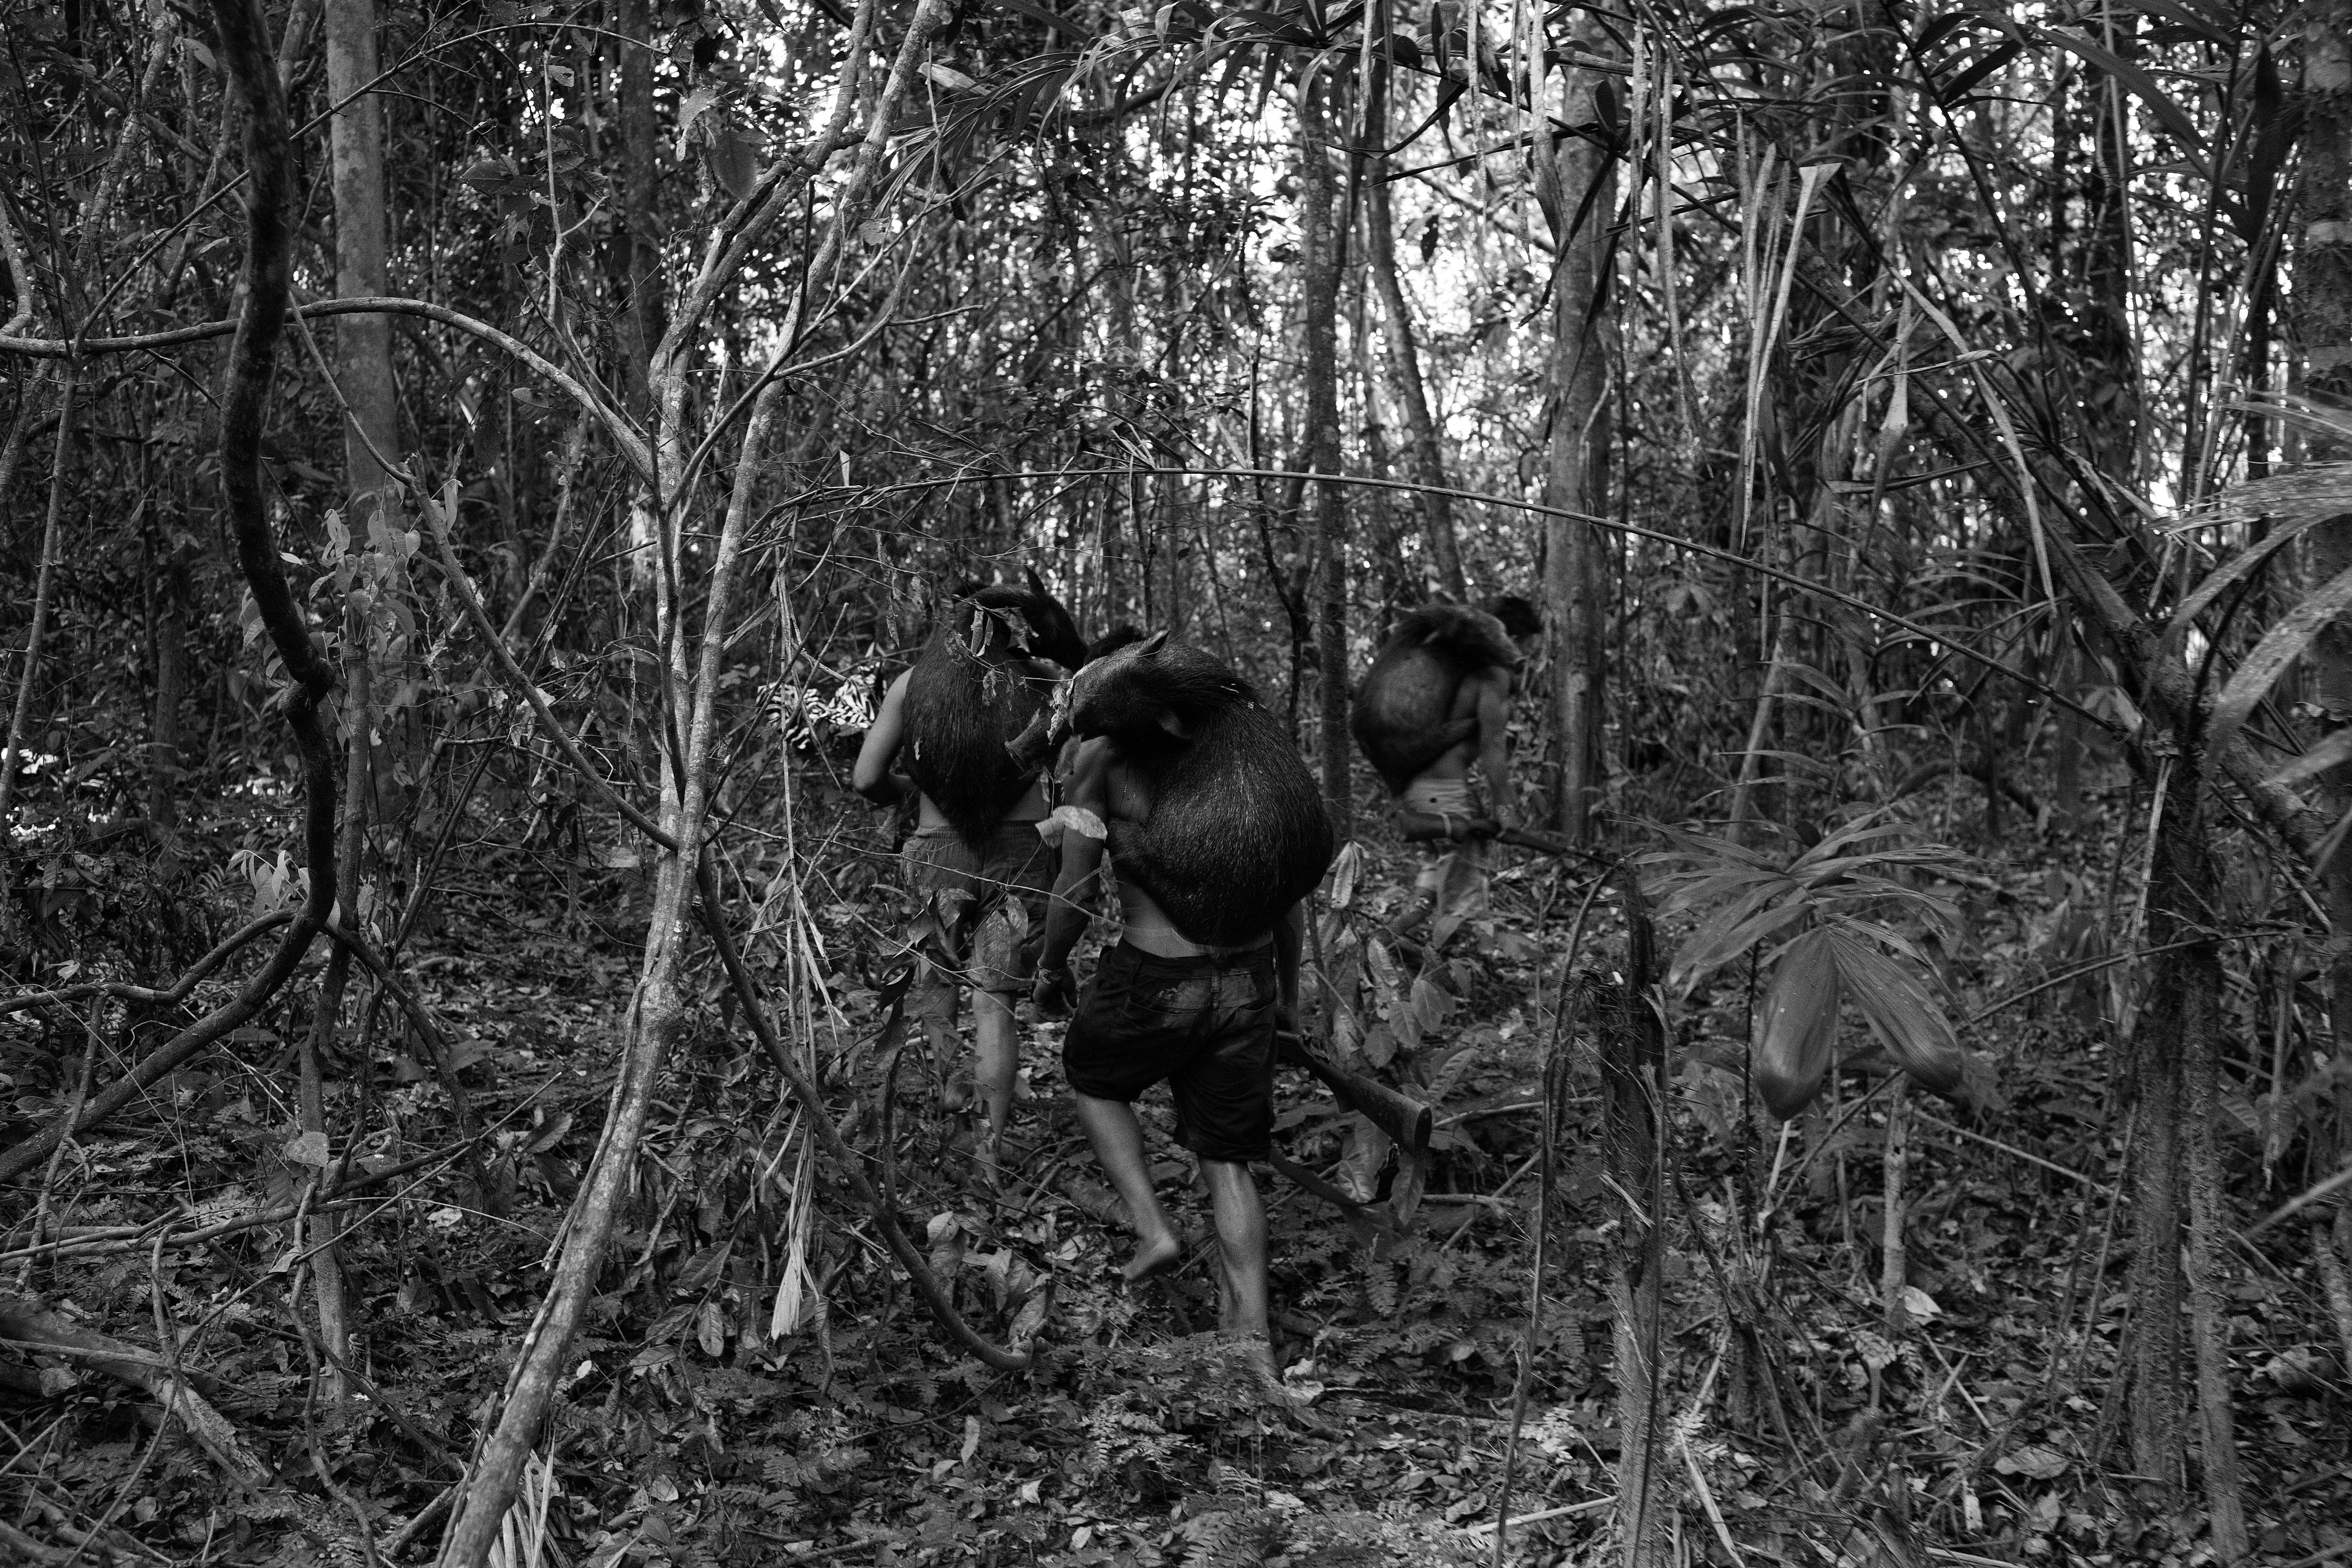
\includegraphics[width=\textwidth]{./imgs/Domenico_V1A8262}
\caption{A volta da caçada de porcos (aldeia Juriti, 2013, foto de Domenico Pugliese).}
\end{figure}

Nos dias atuais, a aldeia Juriti parece ter alguns \emph{harakwaha}
comuns, em que alguns grupos têm privilégio de certos espaços mais
``exclusivos'' para seu uso, em detrimento de outros. Tais escolhas são
determinadas pelo conhecimento pregresso que cada família tem de uma
área, além das novas alianças ocorridas nos últimos anos. Embora
diferentes grupos locais estejam juntos em um novo padrão de vida aldeã,
os \emph{harakwaha} ainda são pensados como áreas ``exclusivas'', onde
porém, devido à nova realidade, famílias que frequentam determinada área
da floresta podem também caçar em outra, quase sempre acompanhando
grupos que ali se relacionam. Isto também é discutido por Cormier quando
define os \emph{harakwaha}, nos dias de hoje, como áreas comuns de
parentes consanguíneos de mesmo sexo (Cormier, \emph{op. cit.} 72--74). É fato
que alguns indivíduos, principalmente os mais velhos, não abrem mão das
áreas que já eram suas antes do contato, como é o caso de um indivíduo
chamado ``Kamara''\footnote{Kamara é o termo utilizado para se referir a
  outros povos indígenas, porém, devido a peculiar onomástica Guajá,
  repleta de apelidos, cujo o esboço apresentarei no capítulo 5, este
  indivíduo ganhou dos membros da aldeia o apelido ``Kamara'', tornando"-se
  este seu nome usual.} que, ao acompanhar o grupo de seu genro nas
caçadas em outras áreas, age como se estivesse prestando serviços: (1)
encontra"-se após a caçada com o grupo de seu genro em um local
previamente combinado a fim de carregar, junto com os outros, a pesada
carga de animais abatidos; (2) ajuda a moquear a caça ainda na floresta
antes de voltar à aldeia; ou ainda (3) ajuda os caçadores com seu
domínio de diferentes técnicas de caça (veremos as técnicas de caça no
capítulo 6). Ao penetrar em outros \emph{harakwaha}, Kamara quase sempre
parece um ``intruso'', ainda que nos dias atuais as comunidades vivam em
aldeias comuns. Por isso, ao caçar no \emph{harakwaha} de outros, um
homem pode fazer as vezes de um ``convidado'', um estranho, um parente
distante (\emph{harapihianã}), pelo que aproveita a boa oferta de carne
daquela área e oferece sua ajuda em troca.

Aos poucos aprendi que os dias ideais são aqueles passados na floresta.
Se um ser humano estiver gozando de boa saúde, há muito pouco a fazer na
aldeia, em comparação com as múltiplas possibilidades que a floresta
oferece. Certa vez, no início do verão em 2007, um grupo liderado por
uma mulher, Amỹ Pirahỹ, me convidou para uma pescaria (\emph{pira ika},
``matar peixes'') em um ponto distante do rio Caru, a algumas horas de
caminhada da aldeia. Amỹ Pirahỹ, embora fosse casada, estava acompanhada
de um jovem rapaz, por quem se enamorara, e de sua filha. Saímos tarde
da aldeia, por volta de 9h30min da manhã, e fui pego de surpresa, pois
me chamaram quando já estavam com o pé na trilha. Diferentemente de
outras expedições --- quando eu sempre levava uma mochila com gravador,
máquina fotográfica, canivete, isqueiro, lanterna, algum papel e canetas
extras, além de barras de cereais, que todos comíamos em algum ponto do
trajeto ---, desta vez, por se tratar de uma breve pescaria com saída da
aldeia já tarde do dia, levei apenas minha pequena câmera fotográfica em
um bolso, além do papel e caneta de sempre, em outro.

Para termos uma ideia, uma caçada curta não dura menos que seis horas e,
em média, ficávamos dez horas na floresta, a fim de obter o mínimo de
sucesso nas empreitadas. Quanto às incursões de pesca, estas ainda eram
novidade para mim, uma vez que sempre pescávamos nos arredores da
aldeia. Após sairmos, já afastados da aldeia por alguns quilômetros,
encontramos com mais um grupo formado por uma mulher e seus dois
maridos, totalizando"-se além de mim: três mulheres, três homens, duas
crianças de colo (uma de cada mulher), além de um cachorro fiel que
farejava tudo o que encontrava pela frente. Os dois homens mais velhos
carregavam seus feixes de flechas e arcos, e Juxa'a, o rapaz jovem,
levava sua cavadeira de metal, um valioso instrumento adquirido após o
contato, utilizado para fazer buracos e fundamental para caçar pacas,
tatus e cotias, ``bichos do buraco'' (\emph{ikwapahara} ``os do buraco'').
Nesta hora percebi que, embora eu tenha sido chamado para uma pescaria,
tratava"-se de uma incursão à floresta com todas as possibilidades que
isso oferece (caça, coleta, pesca, e não só isso). Pude perceber o papel
``secundário'' da pescaria quando ficaram por mais de quatro horas em
volta de um buraco, no encalço de uma cotia que fugira. Na sequência,
achamos o rastro de um veado mateiro (\emph{arapaha}), porém desistimos
de persegui"-lo pois, pelas pegadas (\emph{ipopoera}), ele já devia estar
longe. Após o grupo se dividir, como sempre ocorre nessas caminhadas,
mantive"-me junto às duas mulheres e ao cunhado de uma delas, Kamara,
pescando na beira do rio, enquanto os outros homens (que não quiseram me
levar) foram caçar cotias. Cinco horas foi o tempo que eu e Kamara
levamos pescando, e após duas horas de pescaria as duas mulheres que nos
acompanhavam também saíram para ajudar os outros dois caçadores, também
me deixando sozinho --- como se planejassem sair aos poucos para eu não
sentir que não era bem"-vindo por, possivelmente, atrapalhar a caçada.
Durante as horas em que se ausentaram, as mulheres ainda extraíram
resina de maçaranduba (\emph{mixiranỹkaha}), utilizada como iluminação
noturna das casas, embiras (\emph{iwira}), que são cascas de diferentes
troncos de árvores com os quais confeccionam ``cordas'', além de carás
(\emph{kara}), tubérculos que encontraram em uma capoeira na volta para
a aldeia. Em meio a tudo isso, as duas mulheres que carregavam seus
filhos, ambos com cerca de um ano, os amamentavam de tempos em tempos.

\emph{Wata} é o verbo para se referir a essas jornadas. Traduzido
literalmente por ``andar'' ou ``caminhar'', \emph{wata} não pode ser
compreendido apenas como um movimento pelas trilhas de uma área. Além de
\emph{wata}, temos a forma \emph{wataha}, cuja tradução é ``caminhada'',
muito utilizada para se referirem a uma jornada de um dia na mata.
\emph{Wata} é sinônimo de muitas ações que se desenrolam no decorrer de
uma jornada (andar, caçar e coletar) e exprime a grande caminhada que é
a jornada (\emph{wataha}) em si. Por isso, de forma direta, podemos
afirmar que para os Guajá as atividades de ``andar'' e ``caçar'' podem ser
expressas pelo mesmo verbo, \emph{wata}, uma vez que a forma nominal
pela qual todo homem caçador é referido é \emph{watama'a}, cuja tradução
literal é ``caminhador'' (ou ``caminhante''), mas pode também ser traduzida
por ``caçador''. Em uma aldeia Guajá, ao perguntarmos por alguém que tenha
ido à floresta, independentemente do que essa pessoa tenha ido fazer, a
resposta mais comum \emph{é wata ka'ape}: ``foi andar na floresta''. E, em
uma espécie de equivocação linguística, quando traduzem para o português
o verbo ``andar'' (p.ex. ``fulano saiu para andar'', ``fulano vai para
tal lugar''), usam o ``caçar'' em português, como me falaram certa vez:
``Irakatakoa foi caçar (passear) no povoado de Auzilândia''.

É importante lembrar que caçar, como uma atividade ``genérica'', não
existe para os Guajá. As muitas formas de predar uma caça são referidas
de acordo com o animal a ser caçado, não existindo uma forma canônica.
Como um paralelo, lembro que para diversos povos do noroeste amazônico e
piemonte andino, tais como os Ashuar, Huaorani e Tukano, ``caçar'' é
definido como ``soprar'', uma vez que a zarabatana é o principal
instrumento de caça (Descola, 1998, p. 32). O principal objetivo de uma
caminhada/caçada (\emph{wataha}) é caçar algum animal, de preferência
uma carne gorda (\emph{ikira} ``ser gordo(a)/ter gordura'') e saborosa
(\emph{he'ẽ}, ``ser doce''); para tanto, utilizam o verbo -\emph{ika},
outro com cognatos em línguas da família Tupi"-Guarani. ``\emph{arixoho
wari ikapa!''} ``Vamos matar capelães!'' --- ou porcos, mutuns, pacas,
cotias, ou qualquer outro animal --- é uma forma usual para propor uma
caçada. Quase sempre, ir à mata é ir ``matar'' (-\emph{ika}) uma caça
previamente rastreada, seja por ser a época de frutos específicos de uma
presa, seja porque se sonhou com ela, e isso sempre é formulado a partir
de um ou mais nomes juntos a um verbo (``matar'', ``apanhar'', ``comer''), por
exemplo: \emph{wari ika} (``matar capelães''), \emph{akwixi iká} (``matar
cotias''); ou para a coleta \emph{myky'a pyhy} (``pegar pequis'') ou, ainda
\emph{haira u'u} (``comer mel'')\footnote{Quando vão extrair mel, os Guajá
  dizem ``comer mel'' (\emph{haira u'u}) e não ``coletar mel'' (\emph{haira}
  \emph{pyhy}), uma vez que boa parte dele é consumido no próprio ato de
  coleta, enquanto que o restante (quando há) é levado à aldeia.},
dentre outros. As ações envolvidas no \emph{wata} podem ser a caça,
pesca, coleta de mel e frutos, ou, por exemplo, o reconhecimento de uma
nova área a ser explorada, dentre outras atividades. ``Caçar na floresta''
pode ser formulado de qualquer uma destas maneiras, porém o verbo
\emph{wata} utilizado em sinonímia a ``caçar'' funciona como o
significante para diferentes atividades que envolvem incursões pelo
território. É caça e coleta, mas também pode ser a desculpa ideal, seja
para um encontro romântico ou para um isolamento voluntário com o
intuito de se livrar de alguma chateação.

\emph{Wataha} (a caminhada) sequer pode ser considerada uma
possibilidade técnico"-social exclusiva aos humanos, pois as atividades
de andar, explorar o ambiente e obter alimentos é propriedade também dos
animais. \emph{Wata}, como ideia associada a diversos seres, pode ser
traduzido como ``caminhada e procura (por alimentos)''. Assim, por
exemplo: (1) os \emph{karawara}, caçadores que habitam os patamares
celestes, descem à Terra para ``caçar'' (\emph{wata}), a fim de matarem
(\emph{ika}) presas de sua predileção; (2) as antas, veados e pacas
andam (\emph{wata}) à noite atrás de frutos para comer; (3) os macacos,
que pulam de galho em galho atrás de frutinhas e folhas para a
alimentação, estão em sua caminhada, \emph{wataha}. É comum falarem em
português que ``o veado foi caçar frutos'' (\emph{wata}); ou, ``as
baratas foram caçar migalhas'' (\emph{wata}); e assim será com todos os
seres, com a lógica da ``caça'' (como sinônimo de caminhada e procura)
sendo desempenhada por boa parte dos habitantes do mundo.

Tal como já apresentei, os territórios (\emph{harakwaha}) são recortados
por trilhas, e cada trilha tem sua história particular. Desta forma,
andar (\emph{wata}) --- e não remar ou plantar --- além de ser a única
maneira de encontrar alimentos (\emph{hanimi'ũa} ``minha comida''), é a
forma, por excelência, de viver. \emph{Wata pyry}, ``andar junto'', e
mesmo \emph{riku}, que pode ser traduzido por ``estar junto''/``estar
com alguém'', são expressões recorrentes para exprimir os atos de caça,
seja longe, nos acampamentos (\emph{ka'aripa}, ``casas na mata''), ou em
breves jornadas de poucas horas. Durante uma caçada, nas caminhadas para
locais onde se sabe ou se suspeita haver caça, \emph{wata} será sempre
\emph{wata apajhi}, que pode ser traduzido por ``andar rápido'', ideia
que contrasta com \emph{wata me}, ``andar lentamente'', como se deve
fazer em momentos de descanso, descontração, ou mesmo quando retornam de
uma caçada. É comum em um processo de aprendizado um pai ralhar com seu
filho ou filha pequena durante as caminhadas, \emph{awata apajhi} (ande
rápido!), e mesmo \emph{awyhy} (corra!). Certa vez, vi Piraima'ã dizer
para sua filha de cinco anos ``caminha ligeiro rapaz!'', para aprender a
andar no mato de maneira concentrada e silenciosa. Mas o caminho
(-\emph{pe}) também pode ser uma festa para as crianças. Elas nomeiam
tudo na caminhada: cipó, troncos, folhas, pedras, e os menores perguntam
aos mais velhos os muitos nomes que não sabem. Andando na companhia de
adultos e crianças, elas, como que me apresentando a floresta, me
entregavam tudo o que pegavam pelo caminho para que eu olhasse, tocasse,
cheirasse, tal como as crianças fazem entre elas. Neste registro,
``andar'' é ``caçar'', e vice"-versa, podemos pensar tal ideia não como
passível de duas traduções, mas como uma forma particular de atuar no
mundo, um \emph{andar"-caçar}. Se a atividade de caça é também a produção
de alimentos --- o ``aprovisionamento'' (\emph{procurement}, nos termos de
Ingold, 2000 e Bird-David, 1992)---, ela não existiria sem uma elaborada
produção de sentidos e afetos sobre a caminhada.

\section{Fazer, \emph{japo}}\label{fazer-japo}

Os Guajá desenvolveram uma linguagem de assobios (\emph{opia}
``assobiar'') bastante apurada, muito utilizada em situações de caçada ---
quando a voz humana pode estragar todo o esforço de muitas horas de
procura ---, além de ser um sinal de segurança para quem chega
inesperadamente, sem avisar. Sobretudo no verão, quando as folhas secas
formam um tapete de infinitos tons amarronzados na floresta, o estalar
de folhas e galhos pisados pode ser ouvido a centenas de metros; caso um
grupo ouça algo se aproximando --- sem a certeza do que seja ---, um assobio
correto é de extrema importância para que não haja dúvidas a respeito de
quem esteja chegando. Era assim também para a relação das pessoas dos
diferentes \emph{harakwaha}. Quando um grupo adentrava o
\emph{harakwaha} de outro, devia anunciar a chegada com sons, assobios
ou palavras, a depender da situação. O som é produzido tanto por
assobios, propriamente, quanto com as duas mãos em forma de concha sobre
a boca. Por deter tais técnicas, com códigos estabelecidos pela duração
e altura dos sons, os assobios podem ser ouvidos de longe, e muitas
vezes ``conversas'' (perguntas e respostas diretas basicamente) são
estabelecidas. No entanto, hoje em dia são utilizados somente nas
caçadas, uma vez que as mudanças de território terminaram.

Se aparentemente a cultura material de um povo como os Guajá é
extremamente pobre, isto ocorre somente porque ela não foi observada com
lente apropriada. Mesmo com os facões, machados, cavadeiras, limas e
toda a sorte de utensílios de metais que hoje são fundamentais às
atividades cotidianas, ainda encontramos os muitos utensílios que eram
fabricados antes do contato, a partir de um conhecimento prévio sobre
essas áreas de vida, os \emph{harakwaha}. Os Guajá confeccionam uma
diversidade de utensílios, todos muitos simples e descartáveis, que os
auxiliam durante suas jornadas (\emph{wataha}). Ganchos, bolsas,
amarras, embalagens trançadas, toalhas de folhas, forros, casas, todos
eles, objetos com um curto período de vida e confeccionados com folhas e
madeira frescas, adequadas para determinado fim. Tais utensílios são
feitos durante as caminhadas e descartados após o uso, e talvez esta
seja a maior peculiaridade da tecnologia de objetos dos Guajá. Stearman
(2001, p.41) observa algo semelhante entre os Yuquí, da Bolívia. Como já
afirmei, em poucas horas podem levantar toda uma aldeia, com casas,
cozinhas, bancos para apoio, além de cacimbas para água, áreas limpas
para a manipulação (pelagem, limpeza e corte) de caças abatidas --- tudo
confeccionado com embiras, cipós, troncos e folhas.

Se parte da literatura etnológica tende a classificar povos como os
Guajá como dotados de cultura material rudimentar e simplesmente
``adaptados'' a seu habitat, é preciso lembrar que a tecnologia Guajá só
pode ser percebida no contexto da ação em que ela se desenrola. Só
entendendo isso é possível fazer asserções acerca da tecnologia e das
técnicas produtivas de caça e coleta. Tecnologia, tal como formula
Ingold, ``é uma preocupação ocidental''; outros povos estariam preocupados
com, por exemplo, sistemas rituais ou com a relação entre pessoas,
elaborando complexos sistemas de parentesco, porém ``nem o parentesco nem
a tecnologia fornecem uma escala de complexidade'' (Ingold, 2000, p. 313)
pois ela não é um algo em si. Falar em ``tecnologia'' para os Guajá,
portanto, é perfeitamente coerente e inclui complexidade, sim.

Ao chegarmos pela primeira vez a uma aldeia Guajá, algo que chama
atenção é o fato de não haver quase nenhum utensílio confeccionado por
eles (bancos, redes, potes de cerâmica, cestos), o que nos leva a pensar
que os Guajá convivem bem com a falta de uma série de coisas. Porém, ao
acompanharmos a vida que se desenrola na mata, percebemos que uma outra
forma de produção tecnológica está em operação. E, sob essa ótica, tendo
a afirmar que a cultura material \emph{awa} é vastíssima, está em
conformidade com as possibilidades que a floresta oferece e aliada a seu
grande nível de criatividade. Por exemplo, só de uma sacola trançada
feita para carregar suprimentos e utilizada presa às costas --- exatamente
como uma mochila ---, chamada \emph{marakũa}, podemos encontrar dezenas de
variações, tanto em tamanho quanto pelo material utilizado na confecção.
O \emph{marakũa} pode ser trançado com folhas de diversas palmeiras, e
se carregam nele, principalmente, carne de caça e alimentos coletados.
Porém sua confecção é determinada por diferentes fatores: (1) a
capacidade técnica de quem o trança (homens e mulheres o fazem); (2) as
folhas à disposição --- são usadas folhas de palmeiras, preferencialmente
as do açaí (\emph{jahara}, ``jussara'') por serem mais finas que de babaçu
(\emph{hwa'ĩa}) e de bacaba (\emph{pinawã}), mas não somente; (3) o
tamanho e qualidade da carga a ser carregada; (4) o tamanho e a força da
pessoa que carregará o \emph{marakũa}; (5) a distância do ponto a que se
vai com a carga --- a depender dessa distância, o reforço de amarras e
folhas é maior ou menor. Os \emph{marakũa}, independentemente da função
que exercerão, quase sempre são muito bem confeccionados, e os grandes
podem aguentar até mais que 50 kg. Os \emph{marakũa} ``aparecem'' quando
existe uma carga a ser levada, e conforme essa carga --- a história que a
cerca, a história de quem a carrega e quem fabrica o utensílio --- o
objeto vai variar. Trata"-se de uma cadeia formada por relações entre
pessoas, objetos e lugares --- mais do que um dispositivo mecânico e
impessoal. A tecnologia não pode ser dissociada do ambiente ou da
experiência prática das atividades sociais; ela não existe de maneira
absoluta (Ingold 2000, p. 320--321).

Antes do contato, quando não tinham panelas (\emph{japupua}), conseguiam
cozinhar bacabas (\emph{pinawã}) em recipientes feitos com folhas
frescas. Dentro dessa ``panela'' de folhas, despejavam água e, em seguida,
era posta sobre o jirau (\emph{pakapa'ã}, ``moquém''); em poucos minutos
as bacabas estavam prontas para o consumo. Os Guajá podem sair à mata
com uma pequena faca e voltar de lá carregando o resultado da caçada em
vários objetos que, até então, só existiam na memória e estavam por ser
fabricados na mata. É uma noção de tecnologia que prevê a confecção dos
instrumentos como parte do processo de caça, em que \emph{wata}
(caminhar) é também \emph{japo} (``construir'' --- instrumentos, por
exemplo). Em vez de saírem à caça com todos os utensílios necessários,
estes serão revelados de acordo com a situação.

\section{\emph{Ka'ape}, na mata}\label{kaape-na-mata}

A floresta é um local onde se come bem. Nos acampamentos de caça a
fartura sempre está presente, com grandes quantidades de carne
(\emph{ha'okera}). E são esses os lugares preferidos para estar durante
boa parte do ano. A localização das novas aldeias era decidida a partir
da abundância de recursos próximos. Um grupo local poderia se juntar a
outro por um tempo específico, devido à oferta de alimentos em
determinada área que explorassem. Bacaba, babaçu e carnes eram motivo
para todos estarem juntos (\emph{ikwẽ pyry}). Embora a diversidade de
sabores na dieta seja algo apreciado entre os Guajá, os acampamentos são
muitas vezes montados a partir de uma oferta específica de carne, frutos
ou mel (seja uma área onde se encontrem muitos capelães; um bacabal; ou
árvores repletas de méis doces (\emph{he'ẽ}). Nos dias atuais, as
aldeias dos postos indígenas se transformaram em aldeias"-base, fazendo
com que a múltipla localidade experimentada na antiga vida pré"-contato
se transfira para os acampamentos de caça feitos principalmente durante
o verão (\emph{kwarahya}) --- como já mostrei --- e que ainda obedecem à
lógica dos núcleos familiares que viviam dispersos por diferentes áreas.

Tais características podem ser pensadas junto com a definição que
Viveiros de Castro fornece para a territorialidade Araweté, algo
``aberta''. O autor observa que, até o contato, os Araweté ``não tinham
(\ldots{}) a noção de um domínio exclusivo sobre um espaço contínuo e
homogêneo'' (Viveiros de Castro, 1992, p. 31). A ideia de
\emph{harakwaha} até prescreve de alguma forma a noção de um domínio
exclusivo sobre um espaço contínuo e homogêneo; ainda assim, tal espaço
é um fator limitador para uma territorialidade aberta, uma vez que ele é
constantemente refeito. Além disso, os Guajá, tal como os Araweté, não
parecem ter uma ``geografia mitológica'' com sítios sagrados ou locais
primordiais. Não encontrei qualquer referência sobre a relação entre
determinados lugares com, por exemplo, a origem da humanidade; ou sobre
os feitos extraordinários de \emph{Maira} (como veremos no próximo
capítulo). Ao contrário, acampamentos antigos muitas vezes são \emph{ajỹ
ripa}, ou ``morada dos \emph{ajỹ}'', pois são locais abandonados, seja
pela morte de uma pessoa, seja, como vimos, pela necessidade da mudança.
E são justamente esses os locais que os \emph{ajỹ} preferem.

Se a relação direta entre a morte e os \emph{ajỹ}, como veremos mais
adiante, justifica um antigo acampamento como morada desses fantasmas,
tal configuração não precisa estar presente. Os Guajá defendem que os
\emph{ajỹ} se interessam por tudo o que é humano, pois eles mesmos,
equivocadamente (lembram os Guajá), se consideram seres humanos
(\emph{awa}). Desta forma, qualquer acampamento abandonado, seja por
qual motivo for, lhes serve como casa. As ``casas/acampamentos na
floresta'' (\emph{ka'aripa}), há muito abandonadas, são uma espécie de
simulacro de uma aldeia: tapiris (\emph{tapãj}) com telhados
esburacados, moquéns (\emph{pakapa'ã}) caídos, e sujeira por toda parte.
Os Guajá não se interessam mais por tais espaços e, caso voltem a
utilizar um acampamento abandonado, o refazem completamente (erguendo
novos tapiris e moquéns) ou o endireitam (limpam e reparam com folhas
novas) para que resista ao menos a algumas noites.

Quanto aos topônimos, muitos deles parecem circunstanciais, embora haja
referência a alguns pontos geográficos específicos, como as muitas
serras (\emph{wytyra}) que formam o território; açaizais no interior da
mata; árvores antigas; pontos de coleta de mel; velhos acampamentos;
estes e outros são excelentes localizadores, capazes de exprimir com
precisão pontos onde se queira chegar. Em certa situação, Kamara havia
nos informado sobre uma estrada ilegal aberta por madeireiros a cerca de
cinco quilômetros da aldeia Juriti. Preparamos uma expedição até a
estrada e fomos nos informar com ele onde exatamente ela se situava.
Para localizar os homens com precisão, ele responde que ela terminava
próximo a uma grande árvore de tatajuba (\emph{taryka}) onde alguns
meses atrás Wiraho havia matado alguns capelães, o que serviu como um
localizador perfeito. Tal como a tatajuba, buracos de paca, troncos onde
cotias foram capturadas, brejos onde se caçam poraquês, dentre tantos
pontos ativos e utilizados recentemente, esses espaços vivos da mata são
nomeados e utilizados como referência.

Tais classificações escapariam a uma geografia com imagens fixas,
pré"-estabelecidas, sobre o ambiente. Ao contrário, essas especificações
aparecem e desaparecem a partir da interação dos Guajá e seus
\emph{harakwaha}. Como observa Ingold, ``somos inclinados a pensar a
memória como um depósito de imagens na mente, ao invés (de entender a)
lembrança como uma atividade situada no mundo'' (Ingold, 2000, p. 103). É
como se, no caso Guajá, a localização e a memória sobre o espaço --- além
da própria concepção de espaço --- só fosse possível na interação dos
homens com o mundo, e talvez esta ``poética do habitar'' (\emph{poetics of
dwelling}, Ingold, 2000, p. 110) seja um dos princípios de produção do
\emph{harakwaha}.

Certa noite as pessoas da aldeia Juriti ficaram preocupadas com
Piraima'ã que, fazia muitos dias, não conseguia matar qualquer caça e
mesmo assim insistia em retornar à floresta a cada nova manhã.
``\emph{Panemuhũ}'' \footnote{No capítulo 5 discutirei a ideia de
  \emph{panemuhũ}, que por enquanto podemos traduzir por ``azar na
  caça'', tal como o \emph{panema}, comum em toda a Amazônia, e já bem
  discutido por outros autores (ver Matta, 1973).}, diziam as pessoas da
aldeia para afirmar que Piraima'ã estava sem ``sorte'' (\emph{hapiaryhy},
``sorte'', ``aquele que mata rápido a caça''). Nesta noite especialmente ele
estava demorando muito a voltar. Já fazia mais de 12 horas que ele
estava na mata sozinho, sem sorte, em pleno inverno. Em certas ocasiões,
a demora de um caçador em voltar para casa causa preocupação. Mesmo
considerando que cada caçada é uma surpresa, existem situações de que se
pode esperar o pior. Na situação de Piraima'ã, que estava
\emph{panemuhũ} --- cuja consequência mais drástica era a perda de sua
``alma'' (\emph{hajtekera}) ---, o melhor que podia ter feito era permanecer
em sua rede e não ir caçar, sob risco de se perder ou morrer na
floresta. Certa hora, um homem vai à borda da aldeia, local onde se
inicia a capoeira velha (\emph{koa}) que precede a floresta
(\emph{ka'a}), e, com uma voz bem aguda, grita de forma quase
irreconhecível (ao menos para mim) o nome de Piraima'ã, além de formar
outras frases com sons bem específicos que, pela potência, se espalham
no ar. O caçador pode ouvir esse chamado no raio de alguns quilômetros
e, caso ouça, deve respondê"-lo no mesmo tom para que sua resposta não
seja abafada pelas folhas. Nesta noite Piraima'ã ouviu e respondeu e, à
medida que o tempo passava, sua fala se transformava em um canto,
anunciando sucesso na caça. O medo (\emph{kije}) de algo ruim que lhe
poderia ter ocorrido se dissipou. Esse medo, no entanto, sempre estará
presente na relação entre os humanos e a floresta.

As interações com o ambiente passam por detalhes, e todos eles
constituem o conjunto de ações que formam um \emph{harakwaha},
implicando"-se diferentes modos de comunicação, como a mudança no tom e
altura da voz, assobios diversos ou até mesmo o extremo silêncio. Por
exemplo, conversa"-se muito pouco durante as caminhadas, e quando se fala
é bem baixinho, enquanto que em determinados pontos da floresta
(clareiras e acampamentos, por exemplo), pode"-se falar mais à vontade. E
não são somente pegadas que determinam uma trilha (\emph{pea}
``caminho''), já que povos como os Guajá deixam pouco vestígio na
paisagem. Galhos quebrados, folhas remexidas, pegadas intencionais na
terra e marcações nas árvores são postos a todo tempo para que pessoas
que estejam para trás saibam a direção correta a ser tomada e não se
percam nessas trilhas sutis, invisíveis aos olhos de um estrangeiro.

Os animais fogem insistentemente dos humanos que vivem em seu encalço, e
o medo (\emph{kije}) é o estado em que ficam muitos desses animais ao se
encontrar com os caçadores: capelães e outros macacos, antas, porcos,
caititus, veados, cotias, pacas, dentre tantos outros. Para os humanos
os riscos são outros (como se perder ou ser atacado por fantasmas), por
isso as novas trilhas (\emph{pea}) de um \emph{harakwaha} são caminhos
ligados a outros antigos caminhos, formadas a partir de locais por onde
sempre se caminhou. O território é marcado pela memória, e cada trilha
tem seus pontos de parada para a caminhada quase que pré"-definidos, isto
é, são sempre os mesmos: um grosso tronco há muitos anos derrubado serve
como banco; a beirada de um igarapé ou um antigo acampamento são
utilizados como pontos de parada. Por ser a floresta um local perigoso,
tanto pelos seres visíveis (onças e cobras por exemplo) quanto por
invisíveis (sobretudo os fantasmas \emph{ajỹ}), tais paradas funcionam
como locais certificados contra fantasmas, vinganças mágicas de animais
e outros perigos, sítios onde os riscos são menores justamente por serem
de constante presença humana.

Além das onças e dos \emph{ajỹ}, os anos tornaram inevitáveis os
encontros com os \emph{karai}, os não indígenas. Hoje em dia durante as
caminhadas, eventualmente encontram grupos de caçadores ou vestígios de
invasores que há muito se instalaram em suas áreas. Tais encontros são
bastante tensos, com ameaças de morte por parte dos Guajá que, quando
podem, tomam tudo o que encontram: espingardas, facas, machados, lonas,
matam os cachorros. Os
espaços para circulação em seus \emph{harakwaha} estão cada vez mais
limitados devido a pressões das pequenas comunidades de posseiros
(chamados pelos Guajá de \emph{karai caboclos}), que cultivam roças
dentro das áreas, e madeireiros profissionais, que abrem feridas na
floresta. Alguns anos atrás, por exemplo, um grupo de posseiros que
estava fazendo uma roça na Terra Indígena \emph{Awá} foi surpreendido
por alguns Guajá que, após despi"-los, os levaram até a sede do posto. De
lá, a pedido do chefe de posto, foram poupados e mandados embora mata
afora, e nus. Podemos encontrar hoje, em todas as regiões,
independentemente da aldeia, muitas árvores marcadas por madeireiros,
\emph{ira piro} (``árvore raspada''/ ``sem casca''), como tatajubas
(\emph{Bagassa~guianensis}), pequiás (\emph{Caryocar villosum}) e
maçarandubas (\emph{Manilkara}), nas quais exploradores ilegais fazem
marcações para, em seguida, entrar com as motosserras e tratores. Quanto
ao ciclo sazonal, em relação à caça, por exemplo, os Guajá lembram que,
hoje, animais como os porcos têm aparecido majoritariamente nas
temporadas de chuva, pois a floresta está menos ``mexida''. Enquanto o
verão, período agradável para caçar, se transformou talvez na pior
época, pois os madeireiros estão explorando o território; no inverno,
período de chuva, os madeireiros não atuam tanto, assim os porcos ficam
menos assustados. De acordo com os Guajá, que não deixam de utilizar o
humor para se referir a esses episódios trágicos, os porcos dizem entre
si: ``Os brancos não estão, vamos andar!'' Além disso, meus amigos
sempre lembram que os porcos e veados ainda sobrevivem com a roça
humana, as antas ainda comem as embaúbas que nascem nas capoeiras, porém
os capelães, não. Os capelães, ``animais do alto'' (\emph{ma'amija
watehara}, ``caça do alto''), em oposição a esses ``animais de solo'', ``de
baixo'' (\emph{ma'amija} \emph{wypahara}, ``caça do chão/terra''), precisam
das grandes árvores, pois seu território é no alto (\emph{wate}).

Ocorre aos Guajá nos dias atuais o que parece ser uma constante em
diversos povos amazônicos contemporâneos, em que os territórios
demarcados, quando não estão bastante invadidos, estão ameaçados por
pressões no entorno das terras, o que traz uma limitação dos períodos de
deslocamento e alcance de áreas importantes para a caça e coleta (para
outros exemplos relativos à limitação do \emph{trekking} em povos
caçadores ver Rival, 1999, Lee e Daly, 1999) e restrição de uso pelos
animais. Os pequenos acampamentos, próximos às áreas com grande oferta
de caça e frutos, deram lugar a grandes clareiras onde se formaram as
aldeias, com dezenas de casas, onde vivem até 180 pessoas, cada vez mais
distantes dos locais de caça. No entanto, por serem incapazes de manter
uma vida como horticultores, precisam voltar diariamente ao mesmo
interior da floresta onde outrora viviam. Andam para cada vez mais
longe, para onde a caça se foi.

\section{Tocata e Fuga}

Nos anos que antecederam o contato, os antigos \emph{harakwaha} foram
muito rapidamente desmantelados, fosse pela fuga de grupos que recusavam
o encontro com os \emph{karai}, fosse pela mudança compulsória dos
contatados para novas áreas onde já haviam aldeias nos postos. Esse foi
o caso, por exemplo, da família de Takwarẽxa'a que, em meados de 1990,
escapando de fazendeiros e posseiros, saiu em fuga para muito além de
seu \emph{harakwaha} (e do de seus parentes) e foi parar em fazendas
distantes, na região central do estado do Maranhão. Após encontrados por
moradores locais, foram realocados na atual aldeia Juriti, situada em
uma região que Takwarẽxa'á desconhecia: o \emph{harakwaha} de pessoas
com quem não mantinha qualquer relação.

Uma vez estabelecidas as terras indígenas oficiais, muitos
\emph{harakwaha} desmantelados foram, nos dias de hoje, refeitos. No
caso da aldeia Juriti, Wiraho disse"-me que utiliza
uma parte do antigo \emph{harakwaha} em que sua família circulava --- da
época em que era criança e vivia na mata ---, porém algumas áreas ficaram
distantes para ele: foram invadidas por posseiros ou são estradas
ilegais. Diferentemente de ``territórios tradicionais'', os
\emph{harakwaha} atuais são espaços que podem ser ou não remanescentes
de antigas áreas, compostos por pedaços anteriores --- tal qual uma colcha
de retalhos ---, anexados ao de outros grupos locais que agora vivem
juntos, enquanto que outras áreas foram totalmente perdidas. É fato que
muitos dos \emph{harakwaha} antigos ficaram de fora das demarcações das
Terras Indígenas e hoje são ocupados por povoados e até mesmo municípios
inteiros, como é o caso de São João do Caru. No passado, isso forçou os
grupos que formaram a aldeia Juriti a ir cada vez mais para as
cabeceiras do rio Caru e seus microafluentes.

Se o abandono de uma aldeia em detrimento de uma nova, a cada estação,
fazia parte do padrão de deslocamento \emph{awa}, de sua dinâmica
territorial, a fuga desesperada para qualquer direção, como a que
experimentaram nos últimos 100 anos (e mais fortemente a partir da
década de 1960), não obedecia a qualquer dinâmica, a não ser a da
sobrevivência. Era fugir ou morrer, e muitas vezes morriam fugindo.
Sozinhos ou acompanhados por outras famílias, fugiam do ``catarro''
(\emph{tata}, ``gripe'') e do contato com os \emph{karai}. A perda ou
mudança do que eram antigos \emph{harakwaha}, embora tenha ocorrido de
forma acelerada nas últimas três décadas, é um processo anterior ao
contato oficial e característico dos traumáticos anos que antecederam
esse contato, como apresentei no capítulo anterior. Foram anos de
dispersão, uma época em que os grupos locais partiram para qualquer
lugar; com muitas famílias desfeitas, separadas pela morte; crianças
foram deixadas órfãs, e uma fuga sem destino ocorreu, dando origem a
diversos casos de pessoas encontradas bem longe de seus locais de
origem. Este foi o caso de Karapiru, cuja vida --- desde sua fuga pela
sobrevivência, até ser colocado na aldeia em que vive atualmente --- está
marcada por episódios dramáticos.

Karapiru vivia na região de Porto Franco (ver O'Dwyer, 2001) e em 1978,
após uma chacina que dizimou todo seu grupo local, fugiu de sua região
de origem carregando seu sobrinho. Ele foi encontrado em 1988, 10 anos
após sua fuga, vivendo em uma comunidade na Bahia, a uma distância de
700 km das matas em que vivia (ver Tonacci, 2006 e Toral, 2007). A ``saga
de Karapiru'' (nas palavras de Toral) alcançou uma relativa repercussão
na mídia nacional e internacional justamente por historiar elementos
dramáticos e muito particulares: um ``índio nômade'' que sobrevive
cuidando de uma criança, em seguida falecida; sua adaptação e
readaptação ecológica a novos ambientes, durante uma solitária caminhada
de 10 anos; centenas de quilômetros percorridos; sua acolhida junto a
uma comunidade rural completamente excêntrica a sua antiga vida; e, por
fim, o reencontro com seu filho sobrevivente \emph{Xiramukũ} (ou
``Benvindo Guajá''), 10 anos depois (para mais detalhes sobre esses
eventos, ver Toral, 2007). Indivíduos como Karapiru, que simplesmente
fogem, não é algo raro em noticiários locais e até mesmo nacionais
quando o assunto são os Guajá. E, embora o caso de Karapiru seja, além
de emblemático, muito bem documentado, existem outros casos não menos
dramáticos que mostram certa ``forma Guajá'' (se assim posso afirmar) de
reação às invasões e perdas territoriais, como veremos em mais alguns
exemplos.

É também o caso de Jakarexĩ que, tal como ocorreu a Karapiru, teve seu
grupo atacado em uma emboscada de jagunços, a mando de fazendeiros, e em
decorrência disto fugiu até Minas Gerais, sendo encontrado em
1990\footnote{Não é possível saber quanto tempo Jakaretĩ passou fugindo,
  pois a data de sua fuga é imprecisa.}. Segundo Forline (inf. pess.),
enquanto Karapiru andou aproximadamente 720 km, Jakarexĩ teria se
deslocado por 1.100 km, o que, tal como para Karapiru, se trata de uma
distância muito grande. Se pensarmos que tais distâncias foram
calculadas em linha reta --- a partir da região de origem de ambos
(Amarante do Maranhão) e os municípios em que foram encontrados ---,
poderíamos especular que são ainda maiores, uma vez que as viagens a pé
são repletas de idas, vindas e desvios.

Há ainda a ``proto"-odisséia'' de Xaparamuhũ, ocorrida em 2003 durante os
\versal{VI} Jogos dos Povos Indígenas, em Palmas (Tocantins), quando ele --- que
fazia parte da delegação Guajá dos Jogos --- desapareceu durante três
dias. O fato curioso é que Xaparamuhũ não ``se perdeu'', tal como alguém
que se descuida e, desorientado, se perde de um grupo em meio à
multidão. Xaparamuhũ deliberadamente foi embora com sua bagagem, arco e
feixe de flechas\footnote{As duas vezes em que os Guajá participaram dos
  Jogos Indígenas foram apenas em competições de arco e flecha, e se
  saíram muito bem na \versal{VII} edição dos Jogos, em 2004, realizados em Porto
  Seguro. Daí o motivo de cada indivíduo estar com seu feixe de arcos e
  flechas durante os Jogos de Palmas (2003).}, só encontrado por um
pescador após três dias, na beira do rio Tocantins, onde se alimentava
de peixes. O organizador dos Jogos Indígenas à época, Marcos Terena,
promoveu uma busca com auxílio da Polícia Federal e da imprensa (que
divulgou notícias em âmbito nacional), durante três dias.

Entre os Guajá, assim como em outros povos amazônicos e entre os
próprios Ka'apor (ver Ribeiro, \emph{op. cit.}), um estado de raiva pode
induzir qualquer pessoa --- quase sempre um homem --- a se isolar na
floresta. Durante meu trabalho de campo foram muitas as situações em que
homens deixaram a aldeia movidos pela raiva e, em consequência, por uma
necessidade de se manter sozinhos. \emph{Imahy} pode ser traduzido por
``raiva''\footnote{Embora a tradução literal seja ``produzir dor a si
  mesmo''.}, e quando alguém entra neste estado se torna perigoso; em
caso extremo, pode atentar contra a vida de um \emph{harapihiara}, um
parente próximo. Não é raro um homem --- como que sem jeito para
administrar sua raiva --- realizar um retiro voluntário, que pode durar
desde horas até alguns dias, em um velho acampamento de caça na
floresta. É mais seguro para todos. Enquanto os homens se isolam em suas
redes ou fogem para a floresta, as mulheres em situações de raiva a
demonstram com mais desconforto que seus maridos, algo misturado com uma
profunda tristeza (\emph{imehe}). Choros e gritos são típicos quando uma
mulher está zangada, sendo comum em situações como essas lançarem ao
longe alguns de seus animais de criação, ao mesmo tempo que berram para
descontar sua raiva. No dia a dia, muitos são os motivos para raiva e
tristeza, desde a morte de alguém até coisas aparentemente corriqueiras
que ganham proporções descomunais, como um marido que esteve prestes a
flechar sua mulher, pois esta havia comido um mamão inteiro e não havia
guardado sequer um pedaço para ele. Voltaremos a esse tema adiante.

Raiva (\emph{imahy}), medo (\emph{kije}) e tristeza (\emph{imehe}) podem
causar grandes danos às pessoas. Mesmo não sabendo o que se passava com
Xaparamuhũ naqueles Jogos Indígenas de 2003, especulo que uma confusão
entre tristeza, raiva e medo o moveram a deixar tudo para trás, tal como
fez Karapiru duas décadas antes, para sobreviver. O contato produziu o
mesmo sentimento de raiva, medo e tristeza que conheceram em
adversidades anteriores (como conflitos com inimigos e doenças), porém
com uma intensidade nunca antes experimentada. Para situações limites,
de morte e desespero, como viveu Karapiru e os outros, as soluções
também foram de morte e desespero. A promessa de um novo
\emph{harakwaha} que nunca se restabelece, o novo e desconexo ambiente
em que se instalam (e, surpreendentemente, sobrevivem), os laços sociais
que se afrouxaram inclusive por óbitos de parentes, a sub"-dieta a que
são submetidos, tudo isto levou essas pessoas à destruição ou a uma
superação (não menos brutal). Como adiantei no capítulo anterior, em uma
conversa com Karapiru, quando eu gravava alguns cantos (\emph{ijãnaha},
``o canto dele''), ele contou"-me que havia ``desaprendido'' de cantar.
Inicialmente pensei que estava evitando cantar para o gravador,
diferentemente de todos os outros que faziam questão de cantar para mim.
Eu respondi que ele podia cantar o que quisesse, e caso não quisesse
cantar eu também não me incomodaria. Ele então voltou a repetir que
realmente não sabia cantar, e que havia ``morrido um pouco'' (\emph{manũ
mixika'ĩ}) depois dos 10 anos que viveu afastado de pessoas iguais a ele
(\emph{awatea}, ``humanos verdadeiros'', como veremos mais à frente).
Outras pessoas que estavam conversando conosco perceberam meu espanto ao
encontrar um velho que não sabia cantar e trataram de me confirmar o que
Karapiru havia dito: ``sim, ele morreu um pouco mesmo e, por isso, não
sabe mais cantar'', disse"-me Kamajru.

Karapiru foi recolocado na Aldeia Tiracambu, que está a aproximadamente
490 km de distância de sua região de ``origem''\footnote{Muito
  provavelmente, Porto Franco, o local de dispersão de Karapiru já era
  uma área para onde ele estava fugindo.}, junto a outras pessoas que
até então ele não conhecia, pessoas que herdavam histórias e lugares de
vida muito diferentes dos seus; embora todos fossem \emph{awá}, eram
outros parentes, de outras florestas. Como voltar a ser um \emph{awatea}
(um humano de verdade), capaz de cantar e caçar com propriedade, após
uma epopeia como essa? Se para os Guajá a memória e as ações estão
inscritas neste espaço de conhecimento --- o \emph{harakwaha} ---, a perda
deste lugar primordial não é só uma perda territorial, mas da vida em
si, tal como me sugere Karapiru ao afirmar ter morrido, ainda que um
pouco.

Lastimo não ter conhecido pessoalmente Xaparamuhũ, e com Jakarexĩ falei
muito pouco; porém, tendo em vista que a atitude deles fora algo
sistêmica durante os anos de contato (quando muitos indivíduos fugiam
sós), me parece que tal reação --- que envolve uma fuga ``desorientada'' ---
está relacionada com a possibilidade de restabelecimento de novos
\emph{harakwaha}. Para Karapiru, Jakarexĩ, além de tantos outros
anônimos que morreram fugindo --- sem que tivéssemos a chance de conhecer
suas histórias ---, um dos motivos destas diásporas compulsórias era a
possibilidade de um novo \emph{harakwaha}. Diferentemente da história de
Uirá --- um Ka'apor que, mediante uma situação de desengano envolvendo um
estado psicológico de raiva, melancolia e desespero, abandonou a aldeia
e saiu, em vida, à procura de uma entidade transcendente (\emph{Maira})
e da ``Terra sem Mal'' (a epítome da transcendência messiânica Tupi, cf.
Ribeiro, 1980) ---, os muitos Guajá que simplesmente fugiram, deixando
para trás seus territórios, buscavam restabelecer espaços que já não
possuíam, em novos \emph{harakwaha} que nunca mais encontrariam. Dessa
mesma forma, presumo, o aludido ``nomadismo'' dos Guajá é mais bem
entendido quando a mobilidade espacial é pensada como um processo de
produção e reprodução do \emph{harakwaha}. Se antes --- por conta de
guerras intestinas, morte ou escassez de recursos --- novos
\emph{harakwaha} podiam ser constituídos, desde a chegada do rolo
compressor do Estado as fugas de nada adiantaram e novos
\emph{harakwaha} jamais reapareceram. \emph{Watama'a} (``aquele que
caminha'', caminhantes\footnote{Ingold utiliza o termo \emph{wayfarer},
  cuja tradução pode ser \emph{caminhante}, quando se refere a diversos
  povos caçadores"-coletores que enxergam como sinônimo as ideias de
  ``andar'' e ``viver'' (2007: 75--76). Não curiosamente, os Guajá têm uma
  palavra quase idêntica (\emph{wata ma'a} --- \emph{caminhantes)} para
  ``se definirem'' em relação ao território.}, que fazem e são o caminho),
os Guajá sempre refizeram seus espaços de conhecimento
(\emph{harakwaha}), verdadeiros territórios vitais que em muitos outros
casos não puderam ser refeitos, levando muitas vidas a um trágico
destino. É como se tivessem sido trapaceados por sua própria
territorialidade.

%\section{Variações Tupi}\label{variauxe7uxf5es-tupi}

%Como já vimos, o \emph{harakwaha} não é, em absoluto, um território{,}
%mas antes, uma territorialidade, um local de exercício da vida e que
%pode ser considerado em paralelo com outras ideias, por exemplo, a de
%\emph{tekoa}, consagrada pela bibliografia dos Mbya e Guarani em geral.
%Não tenho elementos para associar o \emph{harakwaha} Guajá com o
%\emph{ethos} buscador guarani (em que a insatisfação pela vida na Terra
%é compensada pela busca de novos lugares onde possam viver bem, sem que,
%na verdade, nunca encontrem local verdadeiramente bom), posso apenas
%traçar algumas associações.

%Em uma definição simplificada, \emph{tekoa} são espaços --- e buscas por
%espaços --- que muitas vezes são sonhados pelos xamãs ``para pôr em prática
%o modo de vida (\emph{teko}) guarani'' (Pissolato, \emph{op. cit.}, p.
%115)\footnote{Para uma discussão completa sobre o \emph{teko} e
%  \emph{tekoa} guarani, ver o balanço de Pereira (2004) e Pissolato
%  (2007: 105--122).}. Nas palavras da autora, \emph{tekoa} é a ``realização
%    de um jeito de ser, um costume, um modo de vida, o que envolve
%    certamente uma dimensão espacial ou, melhor dizendo, espaciotemporal,
%    mas não se define inicialmente por ela''. Embora o \emph{tekoa} guarani
%seja ``a manifestação do \emph{teko}, (um) modo de ser'', esta fórmula
%relacional não remete a um modo plenamente determinado de ser \emph{nem
%implica uma definição precisa de lugar} (Pissolato, \emph{op. cit.}, p. 119,
%meu grifo). Inclusive, linguisticamente as ideias de \emph{tekoá} e
%\emph{harakwaha} são comparáveis, pois, de acordo com Magalhães (2007),
%ambas são oriundas do verbo \emph{iko} ``estar em pé, em movimento'', e
%\emph{tekoa} também pode ser traduzida como ``o lugar de pessoas estarem
%em movimento''. A palavra Guarani de \emph{nhandereko} (``nosso modo de
%ser'') é cognata do \emph{janakwaha}, da língua Guajá (``nosso lugar'').
%Proponho aqui tal relação com essas formas guarani, pois elas não
%traduzem o território como algo \emph{dado}, mas como se feito
%permanentemente. Isso é o \emph{tekoa}. Por isso diversos autores
%propõem que a noção de \emph{tekoa} seja relativizada ``como categoria
%espacial (ainda que a realização de \emph{teko} implique necessariamente
%a dimensão espaciotemporal)'' (Pissolato, \emph{op. cit}), isto é, a
%espacialidade não é o que define o \emph{tekoá}, embora este precise do
%espaço físico para se atualizar.

%Além do \emph{tekoá} Mbya, destaco a noção de \emph{ere"-kohá} dos
%Zo'é\footnote{Que seria em Guajá \emph{arirakwaha} `nosso lugar de
%  estar'.} --- um povo Tupi"-Guarani pouco estudado, habitantes do norte do
%Pará, linguisticamente próximo dos Guajá e dos Mbya. Entre os Zo'é,
%expressões que aludem à vida coletiva em determinado local como
%\emph{piri} (``viver junto, dormir'') e \emph{koha} (``noção relativa à
%realização de um jeito de ser''), além de \emph{jet} (relação de
%apropriação, uso, cuidado, zelo), ``explicam relações (sociais) num
%ambiente ou universo conhecido'' (Havt, 2001, p. 80). Havt encontra entre
%os Zo'e uma definição para \emph{koha} muito próxima da definição
%guarani de \emph{tekoa} (ou \emph{tekoha}), isto é, o ``lugar de
%exercício de um jeito de ser/ viver'' (\emph{idem}).

%Tanto o \emph{koha} (Zo'é ) quanto o \emph{tekoha} (Mbya) fazem
%referência ao que ambas as autoras sugerem ser espaços de atualização de
%um modo de ser, chamados \emph{teko}, no caso Guarani, e \emph{wereko},
%no caso Zo'é. São termos equivalentes linguisticamente e se associam na
%língua com o \emph{hakwaha/ harakwaha} Guajá; porém não defino o
%\emph{harakwaha} como um lugar de ``pôr em prática'' um ``jeito de
%ser/viver'', mas sim, como também sugerem as autoras, um território que é
%suporte para o exercício de relações sociais definidoras, seja de caça e
%coleta, alianças ou rituais. Uma territorialidade cujo espaço não é dado
%\emph{a priori} e que aparece de acordo com as interações entre as
%pessoas, o ambiente e os diversos seres no mundo parece fazer eco entre
%o \emph{harakwaha} Guajá e essas outras formas.

%Suprimido a pedidos do autor

\section{\emph{Wari rakwaha}, lugar de macaco}\label{wari-rakwaha-lugar-de-macaco}

Assim como encontramos em outras etnografias (p. ex. Jara 1991), dentre
outras relações importantes --- como tamanho, hábitos e dieta ---, os
animais (\emph{ma'amijara}, ``caça'' literalmente) são antes pensados a partir do seu etograma, seus repertórios comportamentais, além do local em que vivem. De maneira geral, os ``animais do alto''
(\emph{ma'amija watehara}) são aqueles cuja maior parte da vida se
desenrola no alto das árvores, mesmo que eventualmente possam descer e
correr sobre a terra como fazem os macacos"-pregos em fuga\footnote{Macacos"-pregos,
  diferentemente dos capelães, tem a cauda pouco robusta o que, em caso
  de emboscadas, dificulta a fuga pelo alto das árvores. Quando precisam
  correr mesmo, esses animais se atiram no solo e se espalham pela
  folhagem o mais rápido e distante que conseguem.}. Os mais lembrados
são: macaco"-cuxiú, capelão, macaco"-cairara, macaco"-prego, jupará,
ouriço"-caxeiro (quandú), preguiças, macaco"-da"-noite e saguis. Nesse
grupo de ``animais do alto'' há também pássaros como tucanos, araçaris,
jacus, jacupemba, araracanga, ararajuba e toda a infinidade de
passarinhos. Os ``animais do chão/terra'' (\emph{ma'mija wypahara)}
constantemente lembradas são: queixada, caititu, anta, tamanduá, quati,
onça pintada, suçuarana, veados mateiro e foboca, cotia, paca, diversos
tipos de tatu, dois tipos jaboti, raposa, cachorro"-do"-mato, papa"-mel,
dentre outros menos lembrados. Uma parte desses ``animais do chão'' é
classificada como ``animais do buraco'' (\emph{ma'amija ikwapahara}),
que só costumam sair para andar à noite, e pouco andam durante o dia.
Por exemplo, os Guajá conhecem cinco espécies de tatu: \emph{tatutea}
(``tatu mesmo''/de verdade); \emph{tatupeperehũa} (``tatu peba'');
\emph{tatukajtua} (parecido com ``tatu peba''); \emph{tatuhua} (``tatu
canastra''); e \emph{tatujawara} (``tatu onça''). Além desses tatus, são
``animais do buraco'' (\emph{ma'amijá ikwapahara}) a paca e a cotia. Há
também uma macro"-classificação para os animais aquáticos (\emph{ma'amijá
y'pahara} ``animais da água'') que além de diversos peixes inclui
quelônios (capiningas e tartarugas), jacarés, poraquês e arraias. Além
dessa classificação topológica, os hábitos noturnos e diurnos dos
animais também os define de alguma forma. Antas, pacas, veados, juparás
e todos os ``animais do buraco'' gostam da noite (\emph{wata}
\emph{pyha} ``andam de noite''). O macaco"-da"-noite, dizem as pessos,
diferentemente dos outros macacos que dormem de noite, preferem dormir
de dia. Já os animais que dormem de noite, e preferem o dia (\emph{wata
ikwamehẽ} ``andam de dia'') sempre lembram de diversas espécies de
macacos (com exeção do macaco"-da"-noite), cotias e empenados como o
inhambu.

Se partes da floresta são o \emph{harakwaha} dos humanos, alguns
animais, além de outros seres, possuem seu próprio \emph{harakwaha}.
Esse fenômeno foi antes observado por Cormier, indicando que os Guajá
situam a terra em que vivem os humanos (\emph{wy}) como o
\emph{harakwaha} de \emph{Maíra}, \emph{Mai'irakwaha}, na grafia da
autora (2003, p. 72). No decorrer de meu trabalho de campo, pude
observar que a ideia de \emph{harakwaha} também aparece como uma
tradução Guajá para nossa noção de \emph{habitat}, locais onde os
animais ``gostam'' (\emph{maparahỹ}) de estar. De maneira ainda mais
específica, os cocais da espinhosa palmeira \emph{ju} (Marajazeiro ---
\emph{Pyrenoglyphis maruja}) é o \emph{hakwaha} (``lugar dele'') de
determinada vara de porcos, um \emph{xaho rakwaha}, pois é este o local
onde encontram comida e de que ``gostam''; da mesma forma, a copa das
árvores é o \emph{hakwaha} dos capelães (\emph{waria}), por isso,
\emph{wari rakwaha}; os buracos (\emph{ikwara}) são o \emph{hakwaha} dos
tatus (\emph{tatua}); e as águas, o \emph{hakwaha} do jacaré
(\emph{jakarea}), de poraquês (\emph{manakya}) e capivaras
(\emph{kapijawara}). Os Guajá não se reportam aos \emph{hakwaha}
(``lugar dele'') de todos os animais que conhecem, mas apenas daqueles
pelos quais se interessam; seja porque os caçam ou simplesmente gostam
deles, conhecendo seus hábitos\footnote{Os Guajá chegam a dizer que até
  mesmo os \emph{karai} (não"-indígenas) tiveram suas \emph{karai ka'a},
  ``florestas dos \emph{karai} '', porém as destruíram e, hoje em dia,
  estão interessados em destruir as \emph{ka'a} dos Guajá.}.

Desde os menores seres, como as bravas formigas \emph{tahya} --- que tanto
atrapalham a vida dos caçadores, obrigando"-os a largos desvios ao longo
da caminhada, pois atacam os pés de maneira impiedosa ---, até os grandes
felinos, como a suçuarana e a onça pintada, seres quase absolutos nesse
ambiente, ou mesmo as gigantescas antas, com seu couro impenetrável
mesmo para um tiro, todos têm seu espaço, seus caminhos e seus
territórios. Tal como ocorre aos humanos, para esses animais a escolha
de um \emph{hakwaha} passa pela combinação de hábitos alimentares,
acesso a recursos básicos de subsistência e qualidade do \emph{habitat}
(segurança, conforto, distância segura de predadores, etc.). Tal
combinação de fatores é expressa pela ideia de \emph{maparahỹ},
``gostar''. \emph{Maparahỹ ka'á}, ``(os capelães) gostam da floresta'', é
dito como se explicasse o fato de a floresta ser repleta desses
primatas; bem como os macacos cuxiús (\emph{kwixua}), macacos"-pregos
(\emph{ka'ia}), macacos"-cairara (\emph{ka'ihua}) e mão"-de"-ouro
(\emph{tapajua}). A ênfase na ideia de ``gostar'' explica hábitos,
preferências e atitudes --- dos humanos e de outros seres --- com relação a
sua vida, com a ideia de \emph{maparahỹ}, utilizada em diferentes
exemplos que variam do parentesco à caça.

Certa limitação linguística impossibilitou"-me distinguir formas mais
precisas pelas quais os Guajá expressam a ecologia; por isso, em nossas
conversas, tive de me ater a ideias abstratas, tal como ``gostar''. Apesar
de uma redução de formas complexas do pensamento Guajá, a ênfase à ideia
de ``gostar'' não seria de todo equivocada, uma vez que encontramos em
outros casos etnográficos ideias não muito diferentes para explicar o
porquê da ocupação de determinado sítio, em que o ``gostar'' (em um
sentido forte) é um componente central da espacialidade, tanto dos
humanos quanto dos animais. Os Zo'e, por exemplo, se relacionam com suas
áreas de vida, algo parecido com a concepção dos Guajá. O termo
-\emph{koha}, ``lugares de exercício de um jeito de ser'', pelo qual se
referem a seus territórios, era utilizado ``não só quando falavam de si
mesmos, mas quando falavam de outros seres, com ênfase para algumas
espécies de macacos (coatá, capelão e prego) e em relação aos mortos
(\emph{taiwyt}) (\ldots{})'' (Havt 2001, p. 77). No caso dos Zo'é, a noção de
-\emph{koha} também se aplica a alguns animais, mas não a outros. Por
exemplo, os caititus e queixadas são, segundo os Zo'e, animais que não
possuem \emph{-koha} ou, ao menos, eles não conheciam seu \emph{-koha}
(\emph{idem}). Estas áreas tradicionais de vida Zo'e que, como no caso Guajá,
extrapolam a condição humana são vinculadas às espécies, de acordo com
as características da espécie e do ambiente. A autora menciona que o
-\emph{koha} dos diferentes seres é definido pelas características
ambientais que ligam o espaço a determinado animal, de acordo com
hábitos alimentares que ligam o animal ``dono'' (-\emph{jet}) da área a
determinado local, além dos hábitos de vida, que ligam as espécies a
seus respectivos ambientes. Para a autora, o -\emph{koha} Zo'e pode ser
traduzido de forma simplificada por ``lugar de'' e de forma mais adequada
por ``lugar de exercício de um jeito de ser/viver'', bem próximo do já
apresentado \emph{tekoha}/\emph{tekoá} dos Guarani.

A caçada a determinado animal é entendida, pela ótica da presa, como uma
invasão a seu \emph{hakwaha}. Os Guajá explicam que os capelães
(\emph{waria}) enxergam os humanos como \emph{karai} \emph{caboclos},
termo pelo qual os próprios Guajá se referem aos madeireiros. A forma de
caça aos capelães (que veremos neste livro) consiste basicamente em uma
emboscada aérea, em que os homens sobem às árvores onde os animais se
escondem e lá travam uma pequena batalha. Essa forma (de os Guajá
ocuparem o espaço aéreo dos capelães) faz com que os caçadores sejam
percebidos pelos capelães tal como os Guajá percebem os \emph{karai},
que, por exemplo, abrem estradas nas áreas dos Guajá: ``são madeireiros
que vieram nos matar'', pensam (\emph{imarakwa}) os capelães.

Humanos e animais percebem o espaço de acordo com suas experiências.
Trata"-se de uma territorialidade que, feita e refeita, varia de acordo
com o ponto de vista do sujeito envolvido no processo. Desta forma, as
muitas invasões que ocorrem hoje em seus territórios são vistas como o
fim do \emph{hakwaha} (``lugar dele'') de muitos animais. Esse é um dos
principais problemas relacionados às invasões ilegais e derrubada de
madeiras. Além do óbvio desastre ambiental que todos percebemos, os
Guajá dizem que as espécies animais que não são mortas, fogem à procura
de novos \emph{hakwaha}, mais distantes. Depois do contato, tiveram de
aceitar que os limites colocados pela nova vida vão de encontro a suas
concepções sobre território, constituído agora por rotas fixas que saem
sempre das imediações dos postos indígenas. Os grupos humanos que viviam
dispersos nos diferentes pontos da floresta, cuja troca de objetos,
serviços e cônjuges era feita em encontros destas pequenas aldeias,
quase sempre durante a estação seca, vivem agora confinados em uma
estranha convivência (aos olhos dos Guajá), em aldeias fixas.

\section{Cosmografia}\label{cosmografia}

A Terra, \emph{wya,} tal como nós a conhecemos --- o local onde vivem os
humanos --- é apenas uma pequena parte do universo social que, além de
\emph{wya}, contaria com alguns patamares celestes, os diversos
\emph{iwa} (ou ``céus''), onde habitam os mortos, \emph{karawara},
\emph{tapỹna}, \emph{-nima} (duplos celestes), além de \emph{kamara}
(outros povos indígenas) e \emph{karaia} (não"-indígenas) celestes. Sua
cosmografia conta com um mundo subterrâneo, também chamado \emph{iwa},
onde vive outra humanidade sobre a qual os humanos da Terra pouco sabem.
Essa paisagem seria resultado da separação de um mundo anterior, onde
céu, Terra e sub"-Terra estavam muito próximos, quase confundindo"-se.
Como em diversas sociocosmologias Tupi, os Guajá se referem a uma
separação das camadas cósmicas, cujo resultado principal foi a
``especiação sociológica da Terra'' (Viveiros de Castro, 1986).
Encontrei alguns mitos do ciclo dos gêmeos Tupi"-Guarani (como veremos no
próximo capítulo), além de uma versão sobre o tema do dilúvio, que teria
destruído uma primeira humanidade e configurado o mundo atual.

Os Guajá contam que, no passado, antes da grande separação, a Terra era
um local insuportavelmente quente, esburacado, cujo céu (\emph{iwa}) era
possível tocar levantando apenas os braços. Nessa época, ``o céu era um
pouco mais alto que o telhado de um tapiri'', me disse um homem, e quando
os capelães pulavam de galho em galho pela mata, os Guajá os matavam com
muita facilidade, não precisando subir em árvores para caçá"-los, pois do
chão um caçador conseguia acertá"-los com suas flechas. Muito embora
experimentassem um relativo conforto, devido à abundância e facilidade
em matar caça e conseguir frutos nas árvores de baixa estatura, sofriam
com as altas temperaturas da Terra, que era muito próxima do céu --- um
lugar muito quente ---, acarretando"-se, além de grande desconforto, muitas
queimaduras em suas peles. A Terra era também um local esburacado, cujos
galhos caídos serviam como pontes e pinguelas na travessia de uma
infinidade de grandes fossos e buracos que formavam a superfície. Foi
nessa época que muitas pessoas despencaram para o patamar subterrâneo,
cujo acesso era livre, e jamais conseguiram voltar. Foram esses humanos
(literalmente) decaídos que deram origem à população do patamar
(\emph{iwa}) subterrâneo.

Quem mais sofria com aquele calor eram as mulheres, elas simplesmente o
detestavam, tinham completa aversão à proximidade com o sol. Certo dia
uma esposa pediu ao marido que tomasse alguma providência, pois não
aguentava mais tanto calor:

\begin{quote}
\emph{Meu marido, por que o céu tem que ser tão baixo? Por que aqui na Terra
faz tanto calor? Assim eu não consigo viver, não consigo não.}
\end{quote}

Insatisfeito com o sofrimento de sua esposa --- e com seu próprio padecer
---, o homem pediu ajuda ao pássaro \emph{japu} (japu"-preto,
\emph{Psarocolius decumanus}), que, como tantas outras espécies animais
nesta época pré"-separação, era também humano; seu nome, \emph{Japu
Jará}\footnote{A maioria dos animais míticos (além dos atuais
  \emph{karawara} celestes) é referida pelo designativo \emph{jara},
  comumente traduzido por ``dono'' na bibliografia Tupi"-Guarani, mas que
  aqui aparece com contornos próprios, o que discutirei neste livro.}. E
o \emph{japu}, por saber como fazê"-lo, aceitou elevar"-se ao céu à altura
que permanece até os dias atuais:

\begin{quote}
\emph{Pode deixar, \emph{hary} (vocativo para parente próximo), me elevarei
ao céu para que vocês não se queimem nem sofram mais com todo esse
calor, disse.}
\end{quote}

\emph{Japu Jara} puxou o céu, afastando"-o para longe, bem acima da Terra
(\emph{wate}, ``longe acima''), e isso fez com que as árvores crescessem
mais alto; e, desde então, os homens devem subir até as copas para caçar
os capelães.

Depois desta mudança, \emph{Japu Jara} e sua esposa subiram ao céu,
permanecendo lá até os dias atuais. O pássaro \emph{japu} que ficou aqui
na Terra é o seu \emph{nima} (xerimbabo/ ou mesmo, ``duplo terrestre'',
como veremos). Assim também, outros seres"-animais que aqui eram humanos
e excelentes caçadores foram para o céu, deixando a Terra à humanidade,
aos bichos e plantas. E até hoje a distância entre os patamares celestes
e a Terra é controlada por \emph{Japu} \emph{Jara}. É ele que não deixa
o céu subir demais (nem cair), fazendo com que o cosmos permaneça
estável.

Enquanto o céu subia se desprendendo, muita terra caiu dos patamares
celestes e preencheu os grandes buracos que havia na Terra, encerrando
definitivamente no patamar subterrâneo a população que, antes da
separação, havia caído nos buracos. A terra endureceu, e as pessoas do
subterrâneo não voltaram mais à Terra (\emph{wya}), nem os habitantes da
Terra conseguem mais descer até lá. Desde a separação, me explicaram, a
Terra é um local fresco --- diferente do que era --- com árvores altas onde
vive um grande bando de macacos que lhes servem de alimento. Inclino"-me
a pensar que, de certa forma, tal como ocorrera com os Araweté segundo
Viveiros de Castro (1986, p. 184), os Guajá foram ``deixados para
trás'', ainda que pelo pedido de uma mulher.

Versões de narrativas como esta podem ser encontradas em diversos outros
povos do conjunto Tupi. Os Ka'apor, um povo Tupi"-Guarani habitante da
mesma região, relatam que havia um tempo em que o céu caiu sobre a Terra
e ficou na altura das casas. Essa Terra ficou escura e sem sol até o dia
em que alguns humanos cortaram o céu e, através desse buraco, algumas
pessoas nele adentraram. Neste momento o céu se separou da Terra
novamente e os que entraram pelo buraco estão lá até hoje (Huxley, 1963,
p. 242). A versão Guajá conjuga os temas da ``subida/queda'' do céu com a
do ``mundo queimado'' (aqui associado ao calor do céu), como um dos
motivos causadores da separação entre Terra e céu (para outras versões,
ver Lévi"-Strauss {[}1964{]}, 2004, p. 333--334 e Viveiros de Castro,
1986, p. 189). Na versão Ka'apor o céu cai, enquanto na versão Guajá o
céu, originalmente baixo, se eleva. Além disso, o desconforto derivado
da queda do céu entre os Ka'apor está relacionado à escuridão que foi
gerada na Terra, enquanto que no caso Guajá o céu originalmente baixo
causava desconforto devido ao superaquecimento.

\section{\emph{Iwa}}\label{iwa}

Este é um local relatado como belo, claro, limpo e farto em comida, com
poucas árvores e várias pessoas, e muitos são os grupos de seres que
povoam o \emph{iwa}: parentes mortos, duplos celestes, animais, plantas
e uma infinidade de seres próprios deste lugar, onde os principais são
os \emph{karawara}. Os \emph{karawara} são descritos ``como os \emph{awa}
(humanos) do \emph{iwa}'', os ex"-habitantes da Terra com os quais os
humanos se relacionam de diferentes formas --- continuaremos vendo isto no
decorrer deste trabalho. Diferentemente da \emph{wya} --- a Terra,
descrita como suja e perecível ---, o \emph{iwa} é um local muito
agradável e farto. As poucas árvores que lá existem são baixas
palmeiras, e os frutos gerados por elas, além de estar ao alcance das
mãos, são maiores que os da \emph{wya}. Assim, os inajás (\emph{inajã})
e as bacabas (\emph{pinawã}) do \emph{iwa} são, além de muito carnudos,
alcançáveis ao esticar de um braço.

Se há algum ponto de convergência nos múltiplos pontos de vista que as
pessoas detêm sobre o \emph{iwa} é o superpovoamento deste lugar.
``\emph{Ha'i tete awa}'', essa é a primeira coisa que os Guajá falam para
explicar o céu: ``Há muitas pessoas lá!'', alguém dizia; ``Parece Santa
Inês (a cidade grande mais próxima)!'', comentava outro; ou, ``É maior até
mesmo do que São Paulo!'', afirmava alguém, para que eu realmente
entendesse a dimensão do lugar. Conforme me ensinaram os Guajá, entre os
habitantes que compõem esse local densamente povoado estão diversos
seres: (1) os humanos (\emph{awa}) que já faleceram --- o \emph{iwa} é o
destino \emph{pós"-mortem} de todo habitante terrestre, como veremos; em
linha gerais, uma vez falecida a pessoa é lá ressuscitada, passando a
viver na forma \emph{karawara}; (2) os \emph{Tapỹna} (ou \emph{Tapỹ}),
seres celestes característicos do \emph{iwa} que exercem proeminência
sobre as outras criaturas celestes, referidos também como ``chefes'' ou
``prefeitos'' do céu; (3) diversos \emph{karawara}, espíritos que seriam
potências animais, vegetais ou objetos, que no céu são humanos; (4) e os
\emph{kamara} e \emph{karai} que têm uma boa relação com eles. Nos
capítulos seguintes veremos mais sobre esses seres.

Os patamares celestes (\emph{iwa}) são incontáveis, os humanos não sabem
ao certo quantos níveis existem sobre a Terra. Na subida para o céu
(\emph{oho iwape}) que os homens experimentam, sobretudo com a
\emph{takaja} (que veremos no último capítulo), uma vez no \emph{iwa}
conseguem subir para mais dois ou três patamares a fim de visitar outras
aldeias celestes. Subir mais do que isso torna"-se perigoso por dois
motivos: (1) os homens correm o risco de se perder no caminho de volta,
dada a vastidão desses diversos céus --- Wiraho me conta que os
\emph{karawara} querem levar os homens para diversas aldeias, algumas
muito longínquas, na intenção de deixá"-los vivendo com belas esposas e
comida farta, o que implica morte dos humanos que isso fizerem, pois não
voltarão à Terra; (2) os humanos não têm condições físicas para suportar
o calor do céu, \emph{iwa haku}, capaz de queimar violentamente sua
pele. Quanto mais distante for o patamar celeste, mais quente ele será;
alguns deles são locais impossíveis de atingir devido a esse calor
letal. Os humanos não aguentam o calor do \emph{iwa}, por isso, em suas
viagens --- como no momento ritual da \emph{takaja} --- não podem lá
permanecer durante um longo período de tempo. O local é tão quente que
os \emph{karawara}, seus principais habitantes, precisam descer à Terra
para se banhar e beber água, uma vez que aquela água avermelhada do
\emph{iwa} é imprestável para o consumo. Toda água utilizada pelos Guajá
celestes é retirada da Terra; somente os jacarés (\emph{jakarea}) que lá
vivem suportam a temperatura elevadíssima das águas celestes.

Além dos diversos \emph{iwa} superiores, há aquele inferior com o qual,
diferentemente do céu, os Guajá não mantêm contato desde a época da
separação dos mundos. Este patamar é a morada de diversos seres, entre
eles, \emph{Pira Jara}, uma ``gente peixe'', que são caçadores de nhambus
(\emph{iramũ}) e criam diversos animais, como porcos e antas. Além
desse, há também '\emph{Y Jara}, ``gente da água'', que são caçadores de
porcos e os abatem com flechas de taquara, tal como as dos humanos
(voltarei a discutir a ideia de \emph{jara} nos capítulos subsequentes,
inclusive, a ideia de ``donos'' --- nesses e em outros seres --- porém para os
casos acima a ideia de ``gente'' fornece uma tradução adequada).

Como o patamar inferior à Terra é também chamado \emph{iwa}, traduzir
esse termo por ``céu'' se mostra um equívoco. Por isso, seguindo outros
autores e na falta de termo mais adequado, utilizarei a palavra
``patamar''. É esta composição do cosmos em camadas, tão difundida entre
os Tupi"-Guarani (veja, por exemplo, Gallois, 1988; e Viveiros de Castro,
1986), que ordena a cosmografia Guajá. Muitos patamares acima da terra e
um abaixo formam o mundo. Durante todo o trabalho voltaremos às relações
entre a Terra e os patamares celestes, por isso é necessário
apresentarmos, ainda que incompletamente, estes espaços. No caso dos
Guajá, podemos afirmar que a Terra, \emph{wya}, seria --- em contraste com
o \emph{iwa} --- basicamente o local onde a vida dos humanos se desenrola,
o local onde os Guajá ``vivem'', enquanto o \emph{iwa} seria o seu
destino \emph{post"-mortem} e a morada dos \emph{karawara}, embora os
humanos também o frequentem.

\section{O avesso da Terra}

O esquema do cosmos Guajá é constituído por vários níveis superpostos ---
mas nem sempre em um eixo vertical --- uns aos outros. As distâncias se
contariam tanto no plano vertical quanto horizontal, e o \emph{iwa} não
é somente o céu que vemos daqui (embora esse também seja \emph{iwa}). Os
homens que conseguem viajar até lá --- através da \emph{takaja} --- para
alcançá"-lo devem seguir para o alto e para o leste (na direção em que
nasce o sol). Ao subir pela \emph{takaja} chega"-se a um patamar
intermediário, aquele repleto de água vermelha (\emph{pinỹ}) e quente
(\emph{haku}); uma vez nesse patamar, sobe"-se novamente, agora em
direção ao leste, e lá está a aldeia dos \emph{karawara}. A concepção do
cosmos Guajá é um tanto próxima da forma como os Araweté definem também
sua cosmografia, pois lá, tal como entre os Guajá, ``a representação do
universo como sendo composto de camadas superpostas (\ldots{}) se mostra
inadequada para uma descrição da cosmologia (\ldots{}), os valores verticais
e horizontais do cosmos se misturam, ou interinfluenciam, e as
qualidades simbólicas do espaço distorcem qualquer neutra geometria''
(Viveiros de Castro, op.cit., p. 188--189).

O esquema geográfico do cosmos compreende, além dos infinitos
\emph{iwa}, dois níveis intermediários. Um deles é chamado \emph{uru
ripa} (``a aldeia dos urubus''), e o outro '\emph{ya} (``água'') --- ou ainda
'\emph{ya haku} (``água quente''), '\emph{yramãj} (``grande água''),
\emph{iwa 'ya} (``água celeste''). No caso desta última, o topônimo não é
importante (acredito nem existir) --- cada pessoa se referia com um nome
diferente, e '\emph{ya}, ``água'', é satisfatório. Neste último, as águas
muito quentes têm ``a cor de urucum'', e os únicos habitantes são jacarés
que, junto com os urubus que vivem em um patamar próximo, são os únicos
que bebem desta água. A morada dos urubus é uma espécie de anexo do
\emph{iwá}, bem próximo à Terra, controlado por um urubu celeste de
aparência humana, \emph{Uru Jara}, ``o senhor dos urubus''. Ao sentirem
cheiro de carne podre, os urubus descem para se alimentar e depois
retornam. Diferentemente de mim, os Guajá nunca demonstraram dúvida
quanto ao fato de os urubus que povoam a Terra morarem no céu. Em
determinada situação, algumas pessoas encontraram um ninho com ovos de
urubus no alto de uma embaúba, próxima à aldeia; foi quando perguntei se
os urubus não faziam seus ninhos no céu. Um homem me respondeu
enfaticamente que era óbvio que não (fazendo o meu ceticismo parecer
ainda mais estúpido), que os urubus (\emph{urua}) precisam das árvores
para fazer seus ninhos, e na morada dos urubus (tal como nos \emph{iwa}
acima) não havia árvores para isso. Em outra situação, ao ver alguns
urubus dormindo na copa de uma árvore, fiz insistentemente uma pergunta
semelhante (do tipo, ``por que eles dormem aqui e não no céu, já que
moram lá?'', ou outra tão aparvalhada como esta), e alguém me respondeu
que eles dormem na Terra, mas frequentam a morada dos urubus, inclusive,
alguns dormem no céu.

No que tange à vida social, o \emph{iwa} é habitado por uma boa parte
dos tipos de seres humanos que vivem na Terra, sejam os \emph{awa}, os
\emph{kamara} (outros indígenas) e os \emph{karai} (não"-indígenas). Os
Guajá celestes são chamados \emph{karawara}, uma classe complexa de
seres (que discutiremos em detalhes no capítulo 8) que os humanos
costumam chamar simplesmente por \emph{awa} (humanos). Estes são
descritos como ``belos'' (\emph{parahỹ}), adornados com braceletes e
cocares de penas de tucano; em seus corpos estão coladas penas de gavião
e urubu rei; as mulheres vestem"-se de saias, também trabalhadas com
penas de tucano. Além dos \emph{karawara}, existem os ``não"-indígenas'',
\emph{karai}. Ao descreverem o \emph{iwa}, enfatizavam que há
motocicletas, caminhões, carros, espingardas, munições, e toda a sorte
de objetos que os \emph{karai} fabricam.

Na morada dos ancestrais, as casas são tapiri (\emph{tapãj}), tal como
os existentes na época em que viviam na floresta, antes do contato --- e
que atualmente são construídos na temporada de verão, nos retiros de
caça. São compostos por um telhado de palha (preferencialmente babaçu e
açaí) que recobre toda a estrutura de troncos de madeira presos ao chão
e/ou amarrados nos galhos baixos de árvores. Uma diferença de natureza
entre a arquitetura celeste e a terrestre é que no \emph{iwa} todas as
estruturas de madeira são confeccionadas com uma madeira especial só
existente lá, conhecida como \emph{irananỹ}. Essa madeira, como quase
tudo que há no céu, é de cor branca (\emph{xũ}) e utilizada na
fabricação dos moquéns e casas celestes. Quanto à dieta, ela é idêntica
à dos Guajá, com a diferença de ser bem mais farta: com caça, frutos de
coleta, farinha e cultivares como abóbora, macaxeira, melancia,
mandioca, batata, cará e arroz, todos consumidos pelos \emph{karawara}.
Caça e mel são retirados da Terra, enquanto os cultivares e frutos de
coleta são adquiridos no próprio \emph{iwa}, sempre mais fáceis de
acessar e maiores. As palmeiras (bacaba, inajá, açaí, babaçu), como já
mencionei, são baixas e seus frutos alcançáveis com um esticar de
braços, tal como as árvores frutíferas como caju (\emph{akajua}),
laranja, bacuri (\emph{muukuria}), banana (\emph{makua}), além dos
pequiás (\emph{mykya'a}) que, muito carnudos, têm caroços muito pequenos
e sem espinhos, bem diferentes dos caroços grandes e espinhentos dos
pequis terrenos. Disseram"-me que no céu também torram farinha
(\emph{tarymỹ}), tal como os Guajá, que aprenderam com a Funai.

Esses \emph{awá} celestes (os \emph{karawara}) podem ser desde parentes
mortos até animais \emph{jaras,} cujo estatuto celeste é o de
\emph{harapihiara}, humanos próximos. Só descem à Terra para caçar
durante o dia, e descem à noite apenas nos meses de verão, durante as
cantorias na \emph{takaja}. Mesmo havendo diversas espécies animais no
\emph{iwa}, eles não são caçados, somente criados como animais de
criação ou simplesmente vivem soltos. Cada \emph{karawara} tem uma
especialidade na caça, derivada quase sempre de seu gosto por algum tipo
de carne. Só para termos uma ideia (já que voltaremos ao tema mais
adiante), o \emph{karawara} do tipo \emph{Makaro Jara} (cujo duplo na
Terra é o pássaro \emph{makaro}, pomba"-galega --- \emph{Patagioenas}
\emph{cayennensis}) vem caçar somente porcos queixada, assim como outros
são caçadores especializados em outros animais. São dezenas de
\emph{karawara} que apresentarei no último capítulo. Por ora, só é
importante enfatizar que todos eles têm livre acesso à Terra, onde vêm
caçar sempre durante o dia e depois voltam para ao \emph{iwa} antes de o
sol se pôr. Sua técnica de caça é bem precisa e específica. Além de
serem muito rápidos, suas armas --- flechas (\emph{wy'ya}) e tabocas
(\emph{kĩ}) --- são dotadas de \emph{tata} (fogo/energia)\footnote{A ideia
  de \emph{tata} é utilizada para definir tanto a energia elétrica
  quanto o fogo. Assim, o poraquê (\emph{marakya}), o peixe elétrico
  (\emph{Electrophorus electricus}), seria dotado de \emph{tata}, tal
  como minha lanterna o é. Ao mesmo tempo, \emph{tata} é o vocábulo pelo
  qual denominam o fogo. Ao traduzirem \emph{tata} para o português, por
  vezes era como ``fogo'', por vezes, como ``energia'', a depender da
  situação em questão; porém, se tomarmos o cognato Mbya para fogo
  -\emph{ata}, suponho que a {energia} é vista pelos Guajá como {fogo}.},
proporcionando"-lhes uma vantagem técnica durante a caçada que aniquila a
presa com precisão e rapidez. Alguns deles utilizam espingardas
(\emph{maka}), e seus cartuchos, em vez de chumbo, são compostos de
\emph{tata}. Os humanos não conseguem ver tais caçadores
extraordinários, pois, além de serem muito velozes e eficientes em suas
caçadas, eles descem em locais afastados, dentro da mata, e nunca
coincide que cheguem onde os Guajá estejam circulando. Ao caçarem algum
animal, os \emph{karawara} amarram a presa abatida e voltam ao
\emph{iwa} imediatamente. O trabalho na Terra só consiste em abater.
Todo o processo de ``pós"-caça'' (fundamental para o consumo da carne) ---
despelar (\emph{hape}) o animal (retirar a pele por queima e raspagem
e/ou corte), destripar e moquear --- é realizado no \emph{iwa}. Os
\emph{karawara} não estocam a carne moqueada nem mesmo por um dia
sequer, como fazem os humanos. A carne é partilhada e consumida. Quando
seus filhos voltarem a ter fome, retornam à Terra para uma nova caçada.
Por serem caçadores magníficos, não encontram dificuldade no abate de
novas presas.

No céu também há bichos. Os animais criados no \emph{iwa} são
ligeiramente diferentes dos da Terra. As onças (\emph{jawara}) celestes,
por exemplo, são maiores que as terrenas e muito mais ameaçadoras. No
patamar terrestre, os \emph{jawara} são uma eterna preocupação para os
humanos, sobretudo por sua astúcia e desejo de carne --- fazendo"-os
permanecerem em estado de atenção durante as caçadas. Já no \emph{iwa},
os \emph{jawara} celestes, muito mais robustos que os terrenos, vivem
presos e amordaçados. ``A onça tá amarrada no céu!'', todos costumavam me
dizer. E embora os Guajá me dissessem que as onças do \emph{iwa} são
muito bravas e controladas todo o tempo para não ferir os habitantes
celestes, mesmo assim elas protagonizam cenas de ataques aos Guajá
celestes, oferecendo riscos à vida de muitos seres no \emph{iwa}. Esses
jaguares celestes ainda descem à Terra para capturar porcos e levar ao
céu para se alimentar.

Ainda no bestiário celeste é mencionada uma espécie de macaco capelão
que, diferentemente dos de cor preta (\emph{pinuhũ}) encontrados nos
territórios guajá, seriam vermelhos (\emph{pinỹ}) e só existiriam no
\emph{iwa} (embora haja bugios avermelhados em boa parte da Amazônia).
Ele desce à Terra atrás de frutos e os leva para comer no céu. Este
\emph{waria} (capelão) especificamente é um devorador de humanos, e
encontrá"-lo na floresta acarretaria morte. Além dos habituais bugios de
cor preta encontrados na região, existem variações da cor dessa espécie
pela Amazônia, e a variação ``ruiva'' seria uma delas. Na região dos
Guajá só existem bugios pretos, com as extremidades (patas e pontas do
rabo) levemente douradas. Os capelães inteiramente vermelhos seriam,
para os humanos, animais mitológicos..

Em linha gerais, este é o mundo onde vivem os Guajá. Vejamos agora seus
habitantes.
